%!TEX root = report_template.tex

\documentclass{article}
\usepackage{CJKutf8}
\usepackage{graphicx}
\usepackage{enumerate}
\usepackage{amsmath}
\usepackage{amsthm}
\usepackage{amsfonts}
\usepackage{hyperref}
\usepackage{subfigure}
\usepackage{amsmath}  

\usepackage{geometry}
\geometry{left=3.5cm,right=3.5cm,top=4.0cm,bottom=4.0cm}
\usepackage{times}

\usepackage{indentfirst}

\usepackage{algorithm}  
\usepackage{algpseudocode}  
\usepackage{amsmath}  
\renewcommand{\algorithmicrequire}{\textbf{Input:}}  % Use Input in the format of Algorithm  
\renewcommand{\algorithmicensure}{\textbf{Output:}} % Use Output in the format of Algorithm    
\usepackage{listings}
\usepackage{url}

\usepackage{etoolbox}
\newtoggle{solution}
\toggletrue{solution}
% \togglefalse{solution}

\usepackage{color}
\usepackage[dvipsnames]{xcolor}
\newcommand{\solution}[2][0pt]{\iftoggle{solution}{\smallskip{\color{red}{\flushleft\textbf{Solution}:}\par#2}}{\vspace*{#1}}}

\renewcommand{\baselinestretch}{1.2}%Adjust Line Spacing
%\geometry{left=2.0cm,right=2.0cm,top=2.0cm,bottom=2.0cm}% Adjust Margins of the File

% Create horizontal rule command with an argument of height
\newcommand{\horrule}[1]{\rule{\linewidth}{#1}}
% Set the title here
\title{
    \normalfont \normalsize
    \large \textsc{ShanghaiTech University} \\ [15pt]
    \horrule{2pt} \\[0.5cm] % Thin top horizontal rule
    \huge CS271 Computer Graphics \uppercase\expandafter{\romannumeral 2} \\ % The assignment title
    \LARGE Fall 2025\\
    \LARGE Problem Set 1\\
    \horrule{2pt} \\[0.5cm] % Thick bottom horizontal rule
}
% wrong usage of \author, never mind
\author{}
\date{Due: 23:59, Oct. 24, 2025}

% Add the support for auto numbering
% use \problem{title} or \problem[number]{title} to add a new problem
% also \subproblem is supported, just use it like \subsection
\newcounter{ProblemCounter}
\newcounter{oldvalue}
\newcommand{\problem}[2][-1]{
	\setcounter{oldvalue}{\value{secnumdepth}}
	\setcounter{secnumdepth}{0}
	\ifnum#1>0
		\setcounter{ProblemCounter}{#1}
	\else
		\stepcounter{ProblemCounter}
	\fi
	\section{Problem \arabic{ProblemCounter}: #2}
	\setcounter{secnumdepth}{\value{oldvalue}}
}
\newcommand{\subproblem}[1]{
	\setcounter{oldvalue}{\value{section}}
	\setcounter{section}{\value{ProblemCounter}}
	\subsection{#1}
	\setcounter{section}{\value{oldvalue}}
}

\begin{document}
\maketitle
\vspace{3ex}

\begin{enumerate}
%\item Please write your solutions in English. 
\item Submit your \textcolor{blue}{\textbf{PDF}} solution to the course \textbf{Gradescope}. \textbf{[Code: 8XV4G8]}
\item Submit your \textcolor{blue}{\textbf{Source Code and PDF as a zip file}} to the \textbf{ShanghaiTech EPAN}:  \url{https://epan.shanghaitech.edu.cn/l/RF2KH8}. [\textbf{Filename:} \verb|name_2025xx(your id)_hw1.zip|]
% \item If you want to submit a handwritten version, scan it clearly.
\item There are no restrictions on programming languages.  
\item You are required to follow ShanghaiTech's academic honesty policies. You are allowed to discuss problems with other students, but you must write up your solutions by yourselves. You are not allowed to copy materials from other students or from online or published resources. Violating academic honesty can result in serious penalties.  
\end{enumerate}

\newpage

\problem{Melkman's Algorithm for Simple Polygon Convex Hull}

Implement Melkman's algorithm to compute the convex hull of a simple polygon in $\mathcal{O}(n)$ time complexity.\bigskip

\noindent \textbf{Reference:} Lecture 2, page 71

\noindent \textbf{Requirements:}
\begin{enumerate}
    \item \textbf{Input:} A simple polygon represented as an ordered sequence of $n$ vertices.
    \item \textbf{Output:} The convex hull vertices in counterclockwise order.
    \item Complexity analysis explaining why the algorithm achieves $\mathcal{O}(n)$ time.
    \item Test cases with at least three different polygons.
\end{enumerate}

\newpage

\newcounter{Psec}\setcounter{Psec}{0}
\newcounter{Psubsec}[Psec]\setcounter{Psubsec}{0}
\newcommand{\psec}[1]{\refstepcounter{Psec}\vspace{0.6ex}\noindent\textbf{\thePsec.\ #1}\par\vspace{0.2ex}}
\newcommand{\psubsec}[1]{\refstepcounter{Psubsec}\vspace{0.4ex}\noindent\textbf{\thePsec.\thePsubsec\ #1}\par\vspace{0.15ex}}

\psec{Problem Definition and Notation}

\textbf{Simple polygon.}  
A simple polygon is a closed planar chain formed by connecting a finite sequence of distinct vertices in order such that non-adjacent edges do not intersect.  
It defines a single, non-self-intersecting boundary enclosing a finite region in the two-dimensional Euclidean space $\mathbb{R}^2$.  
Throughout this work, polygons are assumed to be strictly simple and embedded in $\mathbb{R}^2$, consistent with the scope of Melkman’s convex hull algorithm.

\textbf{Convex hull.}  
Given a simple polygon $P$, its convex hull $\mathrm{CH}(P)$ is the smallest convex polygon that fully contains $P$.  
The result produced by Melkman’s algorithm lists the hull vertices in counterclockwise (CCW) order.

\textbf{Remark.}  
Since the \emph{Input} and \emph{Output} have been formally defined in the problem statement, they are not repeated here.

\textbf{Notation.}  
The primary symbols used in this report are summarized in Table~\ref{tab:notation1}.

\begin{table}[H]
\centering
\caption{Notation used in Problem~1.}
\label{tab:notation1}
\renewcommand{\arraystretch}{1.1}
\begin{tabular}{p{5.0cm} p{8.3cm}}
\hline
\textbf{Symbol} & \textbf{Description} \\
\hline
$P = (p_0, p_1, \dots, p_{n-1})$ & Ordered vertex sequence representing the boundary of a simple polygon. \\[2pt]
$p_i = (x_i, y_i) \in \mathbb{R}^2$ & Cartesian coordinates of the $i$-th vertex. \\[2pt]
$H = (h_0, h_1, \dots, h_{m-1})$ & Output convex hull vertices in CCW order. \\[2pt]
$\text{orient}(a,b,c)$ & Signed area function determining relative orientation of three points: 
\[
\text{orient}(a,b,c) = (b_x - a_x)(c_y - a_y) - (b_y - a_y)(c_x - a_x)
\]
Positive $\Rightarrow$ $c$ lies to the left of $\overrightarrow{ab}$; negative $\Rightarrow$ right side; zero $\Rightarrow$ collinear. \\[6pt]
$|P| = n,\ |H| = m$ & Number of vertices in the polygon and in its convex hull. \\
\hline
\end{tabular}
\end{table}

\psec{Data Structures and Algorithm}

\psubsec{Data Structures}

The algorithm takes an ordered vertex sequence 
\(P = (p_0, p_1, \dots, p_{n-1})\), 
where each vertex \(p_i = (x_i, y_i) \in \mathbb{R}^2\) defines the polygon boundary and is accessed sequentially.

A double-ended queue \(D\) maintains the evolving convex hull, storing the upper and lower chains simultaneously.  
Its front represents the head of the upper chain, and its back the tail of the lower chain.  
Each element of \(D\) is a vertex of \(P\), supporting constant-time insertion and deletion at both ends:
\[
D = [d_0, d_1, \dots, d_k], \quad d_i \in P.
\]
This structure enables dynamic updates that preserve the left-turn property of convexity, and the final contents of \(D\) form the convex hull in counterclockwise order.

\psubsec{Algorithmic Overview}

Melkman’s algorithm computes the convex hull of a simple polygon in one linear scan of its ordered vertices.  
A double-ended queue \(D\) maintains the current convex boundary, storing the upper and lower chains simultaneously.  
The first three non-collinear vertices \((p_0,p_1,p_2)\) are oriented counterclockwise to initialize \(D\) with \(p_2\) duplicated at both ends.  
For each subsequent vertex \(p_i\), the algorithm checks whether \(p_i\) lies inside the existing hull—left of both boundary edges.  
If so, it is skipped; otherwise, vertices violating convexity are removed from the deque’s ends before inserting \(p_i\) at both sides.  
Each vertex is processed once and updated a constant number of times, ensuring overall linear-time complexity.

\begin{algorithm}[H]
\caption{Melkman’s Convex Hull for a Simple Polygon}
\begin{algorithmic}[1]
\Require Ordered vertices \(P=(p_0,p_1,\dots,p_{n-1})\)
\Ensure Convex hull \(H\) in counterclockwise order

\If{\(\text{orient}(p_0,p_1,p_2)>0\)} 
    \State \(D\gets[p_2,p_0,p_1,p_2]\)
\Else 
    \State \(D\gets[p_2,p_1,p_0,p_2]\)
\EndIf

\For{\(i=3\) to \(n-1\)}
    \State \(p\gets p_i\)
    \If{\(\text{is\_left}(D[-2],D[-1],p)\)\textbf{ and }\(\text{is\_left}(D[0],D[1],p)\)} \State \textbf{continue} \EndIf
    \While{\(\text{is\_right\_or\_on}(D[0],D[1],p)\)} \State \(D.\text{popleft}()\) \EndWhile
    \State \(D.\text{appendleft}(p)\)
    \While{\(\text{is\_right\_or\_on}(D[-2],D[-1],p)\)} \State \(D.\text{pop}()\) \EndWhile
    \State \(D.\text{append}(p)\)
\EndFor
\State \(D.\text{pop}()\); \Return list of vertices in \(D\) (CCW)
\end{algorithmic}
\end{algorithm}

\psec{Test Case Design}

\psubsec{Special Conditions}

To ensure robustness, representative input configurations are identified to capture the main geometric and numerical challenges of convex hull construction.  
Nearly collinear vertices test orientation stability when \(\text{orient}(a,b,c)\!\approx\!0\), verifying consistent handling of degenerate edges.  
Concave polygons with pocket structures examine bidirectional deque updates and confirm that convexity is preserved under pruning.  
Near-contact edges assess numerical tolerance to minimal gaps and floating-point precision.  
Polygons dense in interior vertices but sparse on the boundary test skip efficiency and validate linear-time behavior.  
Finally, clockwise-ordered inputs confirm correct orientation detection and consistent counterclockwise hull output.  
These scenarios collectively define the space of valid yet challenging inputs against which the subsequent test cases are designed.

\psubsec{Case Design}

\textbf{Case 1: Collinear Band with Near-Degenerate Contact.}  
This case tests numerical robustness under near-collinear and near-degenerate conditions.  
A polygon is constructed with long nearly collinear edge sequences forming a narrow horizontal band, introducing repeated evaluations where \(\text{orient}(a,b,c)\!\approx\!0\).  
A slight geometric perturbation produces a near-contact vertex pair without actual intersection, stressing orientation precision and deque updates at the limits of floating-point resolution.  
The configuration validates stable initialization, consistent inside-tests, and correct maintenance of convexity when handling nearly degenerate geometry.

\textbf{Case 2: Dual-Pocket Polygon for Deque Update Validation.}  
This case examines the correctness of bidirectional deque updates during hull maintenance.  
A polygon containing two concave pockets on opposite sides is designed to trigger front and back popping alternately while preserving overall simplicity.  
The structure forces repeated convexity restoration from both ends, confirming the stability of update order, termination conditions, and boundary consistency throughout incremental hull construction.

\textbf{Case 3: Interior-Point Skipping and Sparse Expansion.}  
This case evaluates efficiency and correctness under mixed interior–exterior vertex distributions.  
A polygon combining dense interior vertices with sparsely distributed exterior ones is used to test skip logic and selective hull expansion.  
The setup ensures that interior vertices are efficiently ignored while exterior points trigger minimal necessary deque modifications.  
The configuration confirms that Melkman’s algorithm preserves linear-time behavior and produces a minimal convex boundary even under highly unbalanced vertex distributions.

\psubsec{Visual Summary and Case Coverage}

\begin{figure}[H]
    \centering
    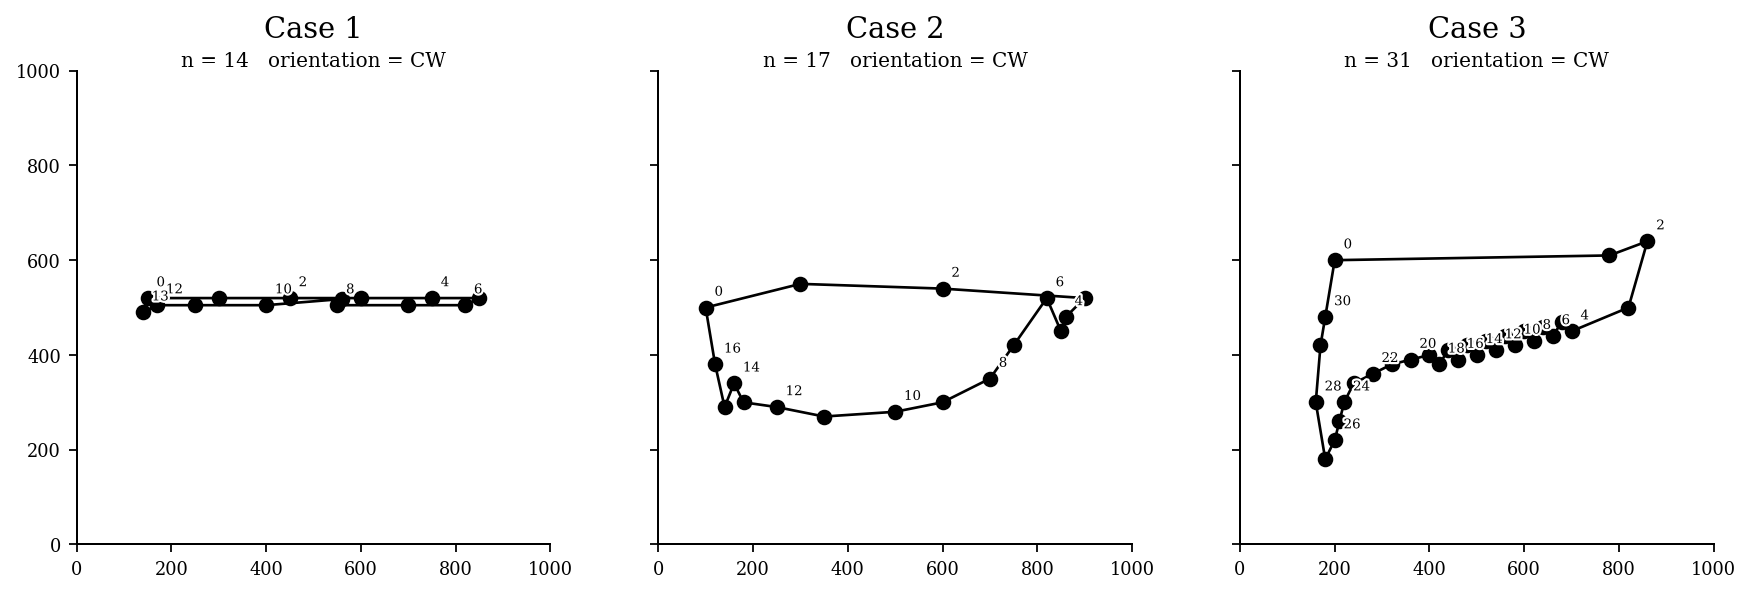
\includegraphics[width=0.9\linewidth]{Pictures/polygon_cases.png}
    \caption{Representative polygon cases used for testing Melkman’s algorithm. 
    Case~1: collinear band with near-degenerate contact; 
    Case~2: dual-pocket polygon; 
    Case~3: interior-point skipping with sparse expansion.}
\end{figure}

The three designed polygons collectively capture the principal geometric and numerical challenges in convex hull construction.  
Case~1 examines stability under near-collinearity and near-degenerate geometry, validating robustness of orientation and convexity maintenance.  
Case~2 stresses deque update correctness through alternating concave pockets, verifying structural consistency during bidirectional hull adjustments.  
Case~3 evaluates efficiency under mixed-density inputs, confirming that interior points are correctly skipped while exterior vertices trigger controlled hull expansion.  
Together, these configurations comprehensively test initialization, inside-testing, and deque-update behavior, demonstrating that Melkman’s algorithm maintains geometric correctness and linear-time performance across all representative input conditions.

\psec{Visualization and Results Analysis}

\begin{figure}[H]
    \centering
    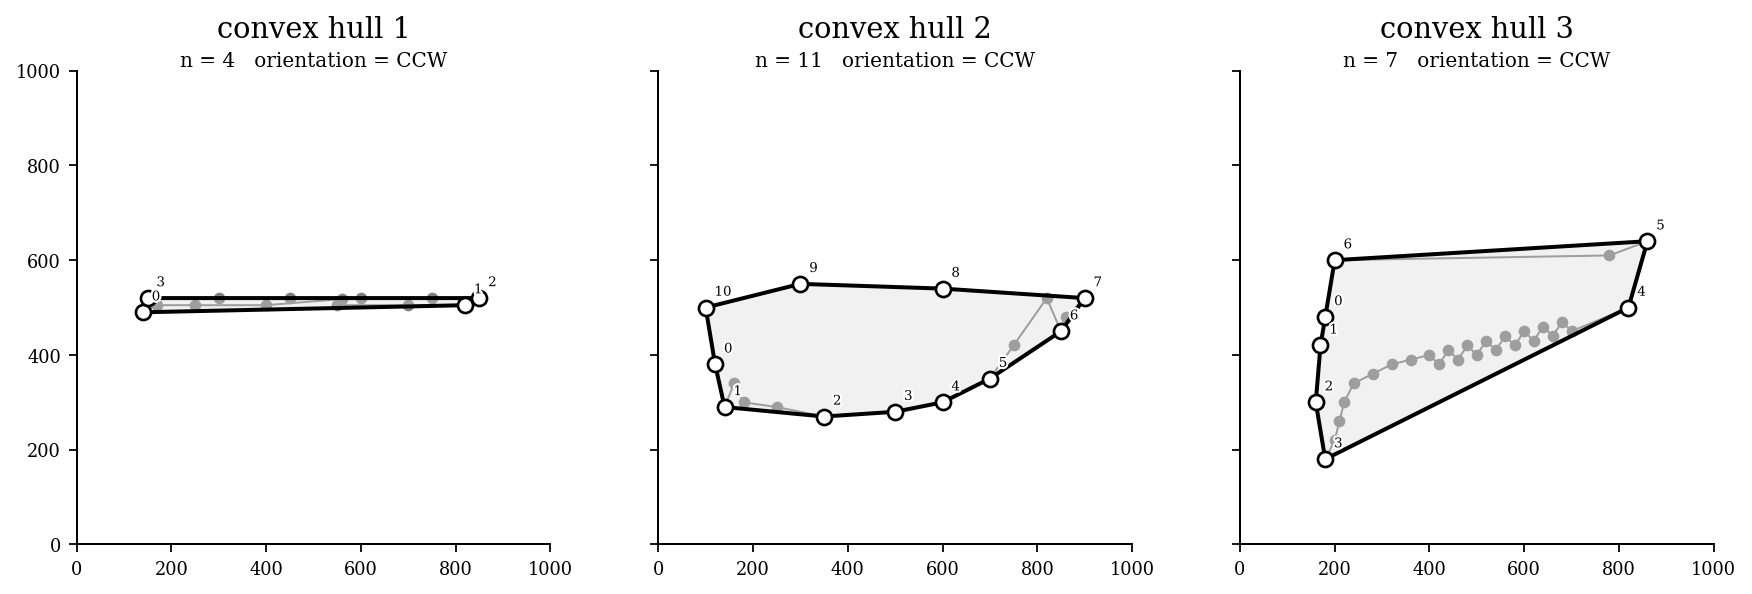
\includegraphics[width=0.95\linewidth]{Pictures/hulls.png}
    \caption{Convex hulls produced by Melkman’s algorithm for the three designed polygon cases. 
    Gray lines denote input polygons; bold black outlines represent computed convex hulls labeled in CCW order.}
    \label{fig:hulls}
\end{figure}

The visualization results confirm the correctness and stability of Melkman’s convex hull algorithm across all representative input categories.  
In the near-collinear case, only the extreme vertices are preserved, demonstrating precise orientation evaluation under near-degenerate conditions.  
In the dual-pocket case, alternating concave indentations trigger consistent deque updates, maintaining convexity and counterclockwise order throughout the construction process.  
In the mixed-density case, interior vertices are efficiently skipped while exterior ones correctly expand the boundary, verifying both logical efficiency and linear-time behavior.  
Overall, the generated hulls are geometrically consistent, free of self-intersections, and fully aligned with theoretical expectations, confirming robustness and correctness of the implementation.

\psec{Time Complexity Analysis}

\psubsec{Theoretical}

Melkman’s algorithm operates in linear time with respect to the number of input vertices.  
Each vertex is processed exactly once during the single forward scan of the polygon and participates in a constant number of orientation checks and deque operations.  
A vertex may be inserted and removed from either end of the deque at most once, ensuring that total operations remain proportional to \(n\).  
The orientation computation \(\text{orient}(a,b,c)\) requires constant-time arithmetic, and no nested or repeated traversals occur.  
Consequently, the overall runtime satisfies
\[
T(n)=c\,n=\mathcal{O}(n),
\]
where \(c\) denotes the aggregate constant cost of orientation evaluation and deque maintenance.  
This guarantees optimal linear-time performance for convex hull construction on simple polygons.

\psubsec{Empirical}

To experimentally verify the theoretical linear-time complexity of Melkman’s algorithm, a controlled evaluation was designed to measure how runtime and operation count scale with problem size.  
From a theoretical standpoint, if the algorithm is truly \(\mathcal{O}(n)\), the total execution time \(T(n)\) should increase linearly with the number of input vertices \(n\), since each vertex is processed once with constant amortized cost for orientation testing and deque updates.  
Accordingly, the experiment quantifies empirical complexity through two measurable quantities: the total runtime and the total number of elementary operations (orientation, cross-product, and deque operations).

The problem size was parameterized by polygon vertex count, with a series of test sets generated at progressively increasing sizes to ensure sufficient geometric diversity while maintaining comparability.  
Each polygon serves as an independent trial for a given \(n\), and both execution time and operation statistics were averaged across runs for stability.  
The generated polygons and their corresponding convex hulls are shown in Figures~\ref{fig:testpolys} and~\ref{fig:testhulls}, all of which were visually verified for correctness prior to measurement.

\begin{figure}[H]
    \centering
    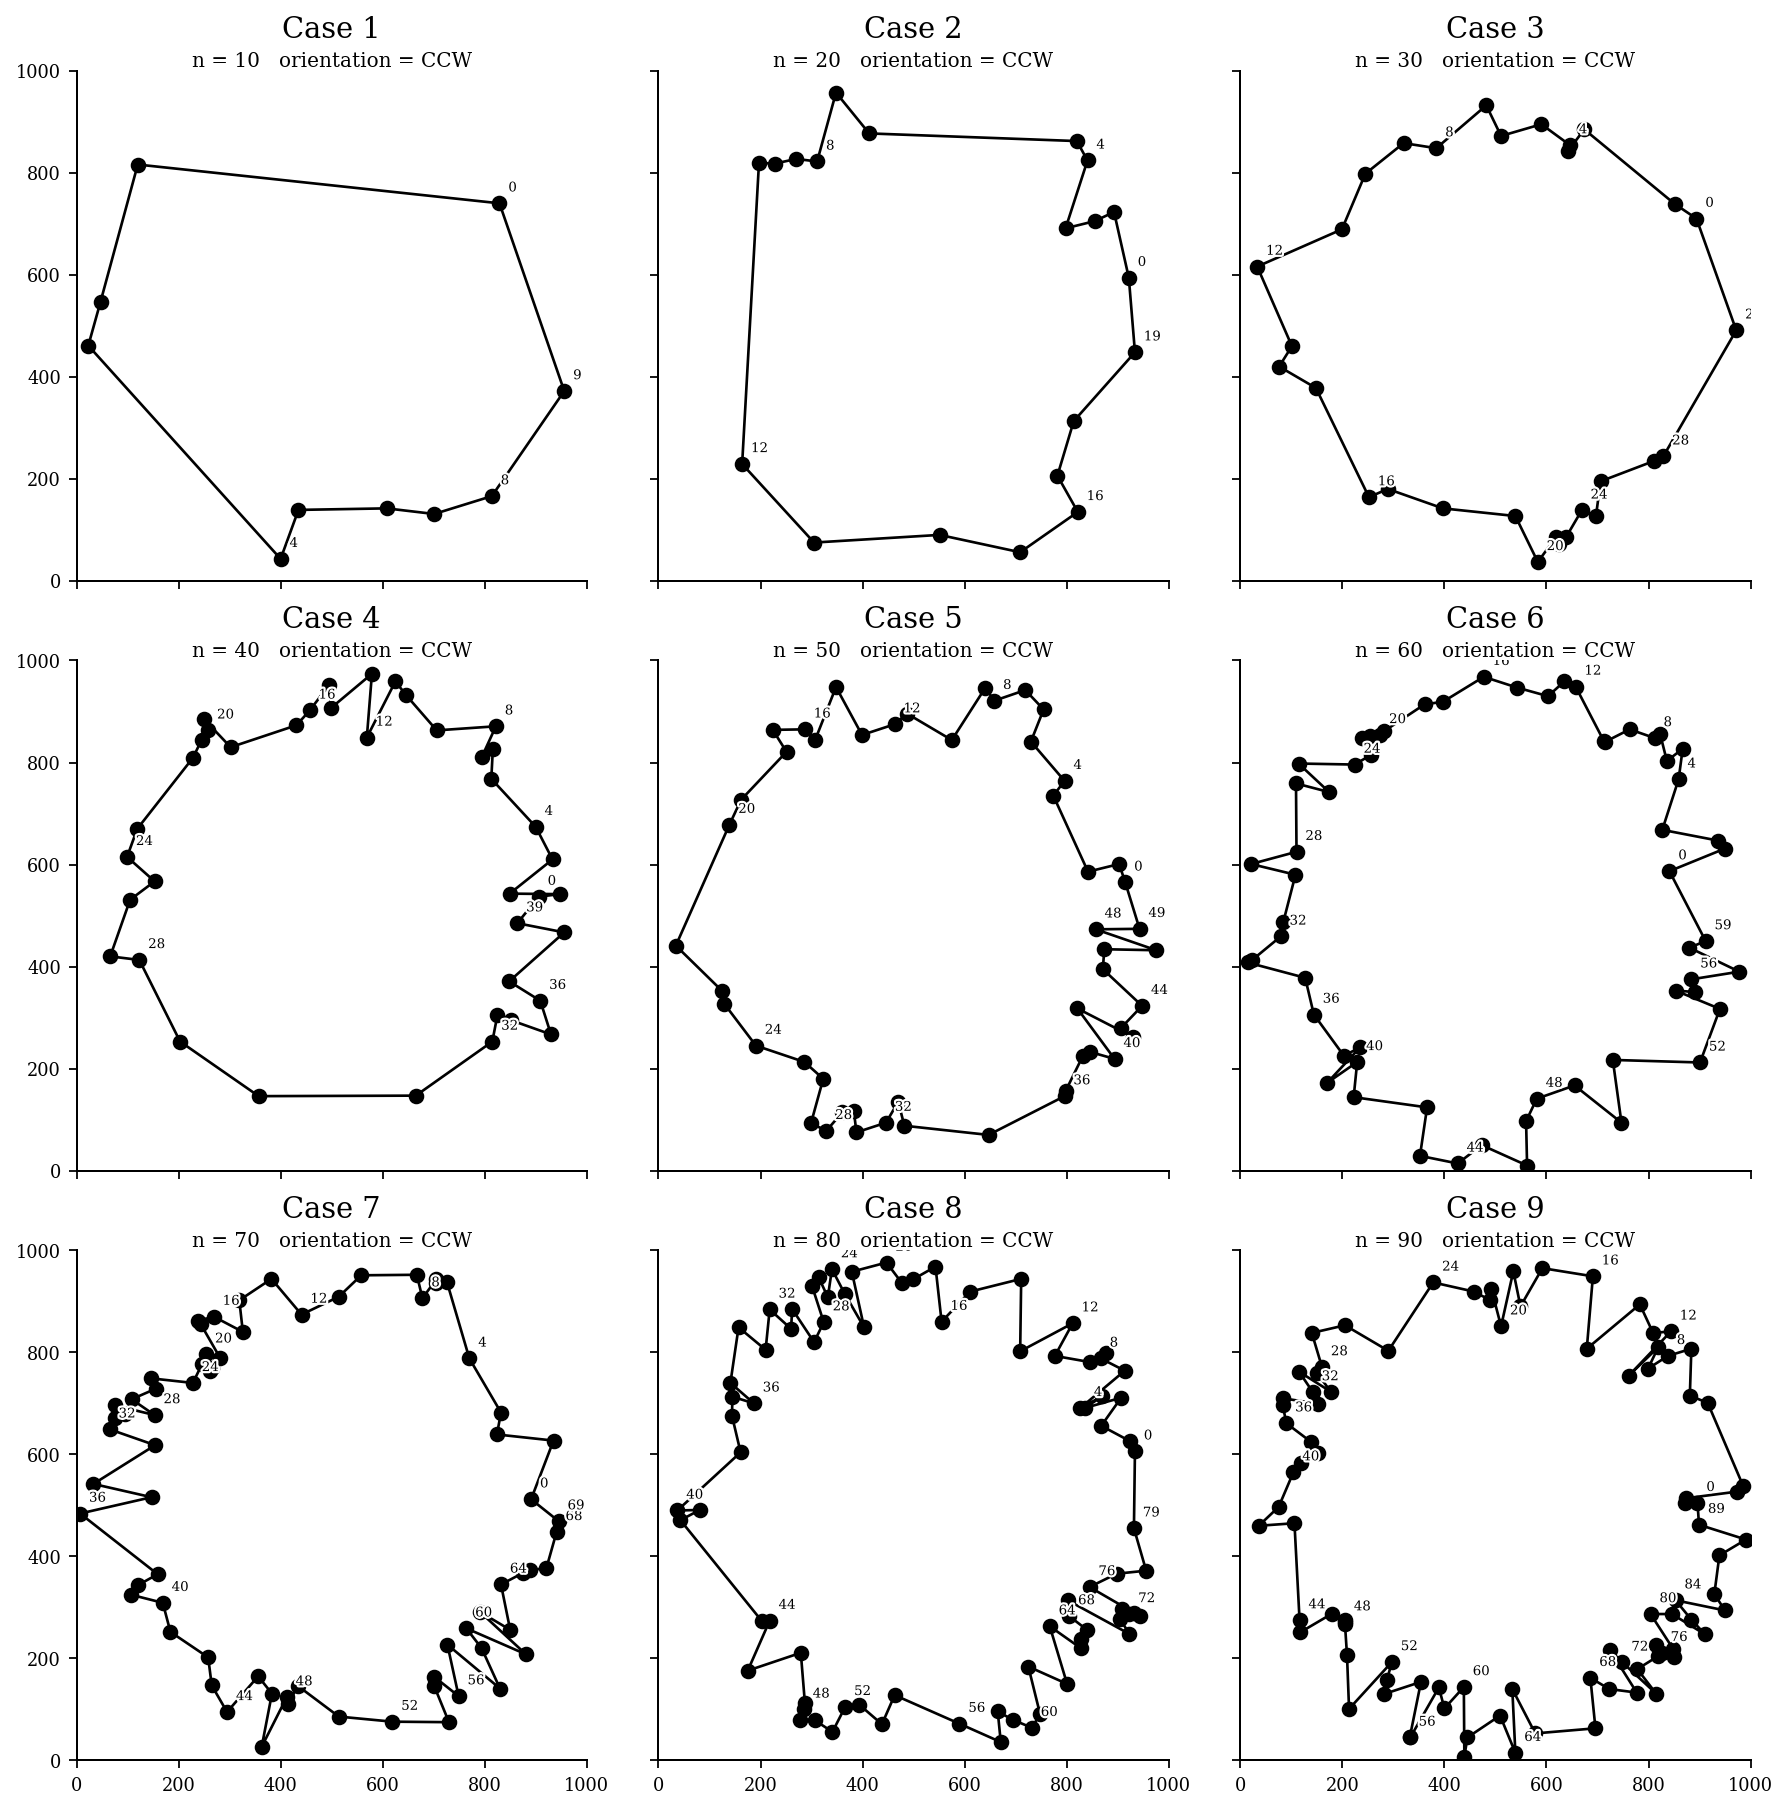
\includegraphics[width=0.95\linewidth]{Pictures/test_polygon_cases.png}
    \caption{Generated polygon inputs with increasing vertex counts ($n=10$–$90$) used to evaluate empirical time complexity.}
    \label{fig:testpolys}
\end{figure}

\begin{figure}[H]
    \centering
    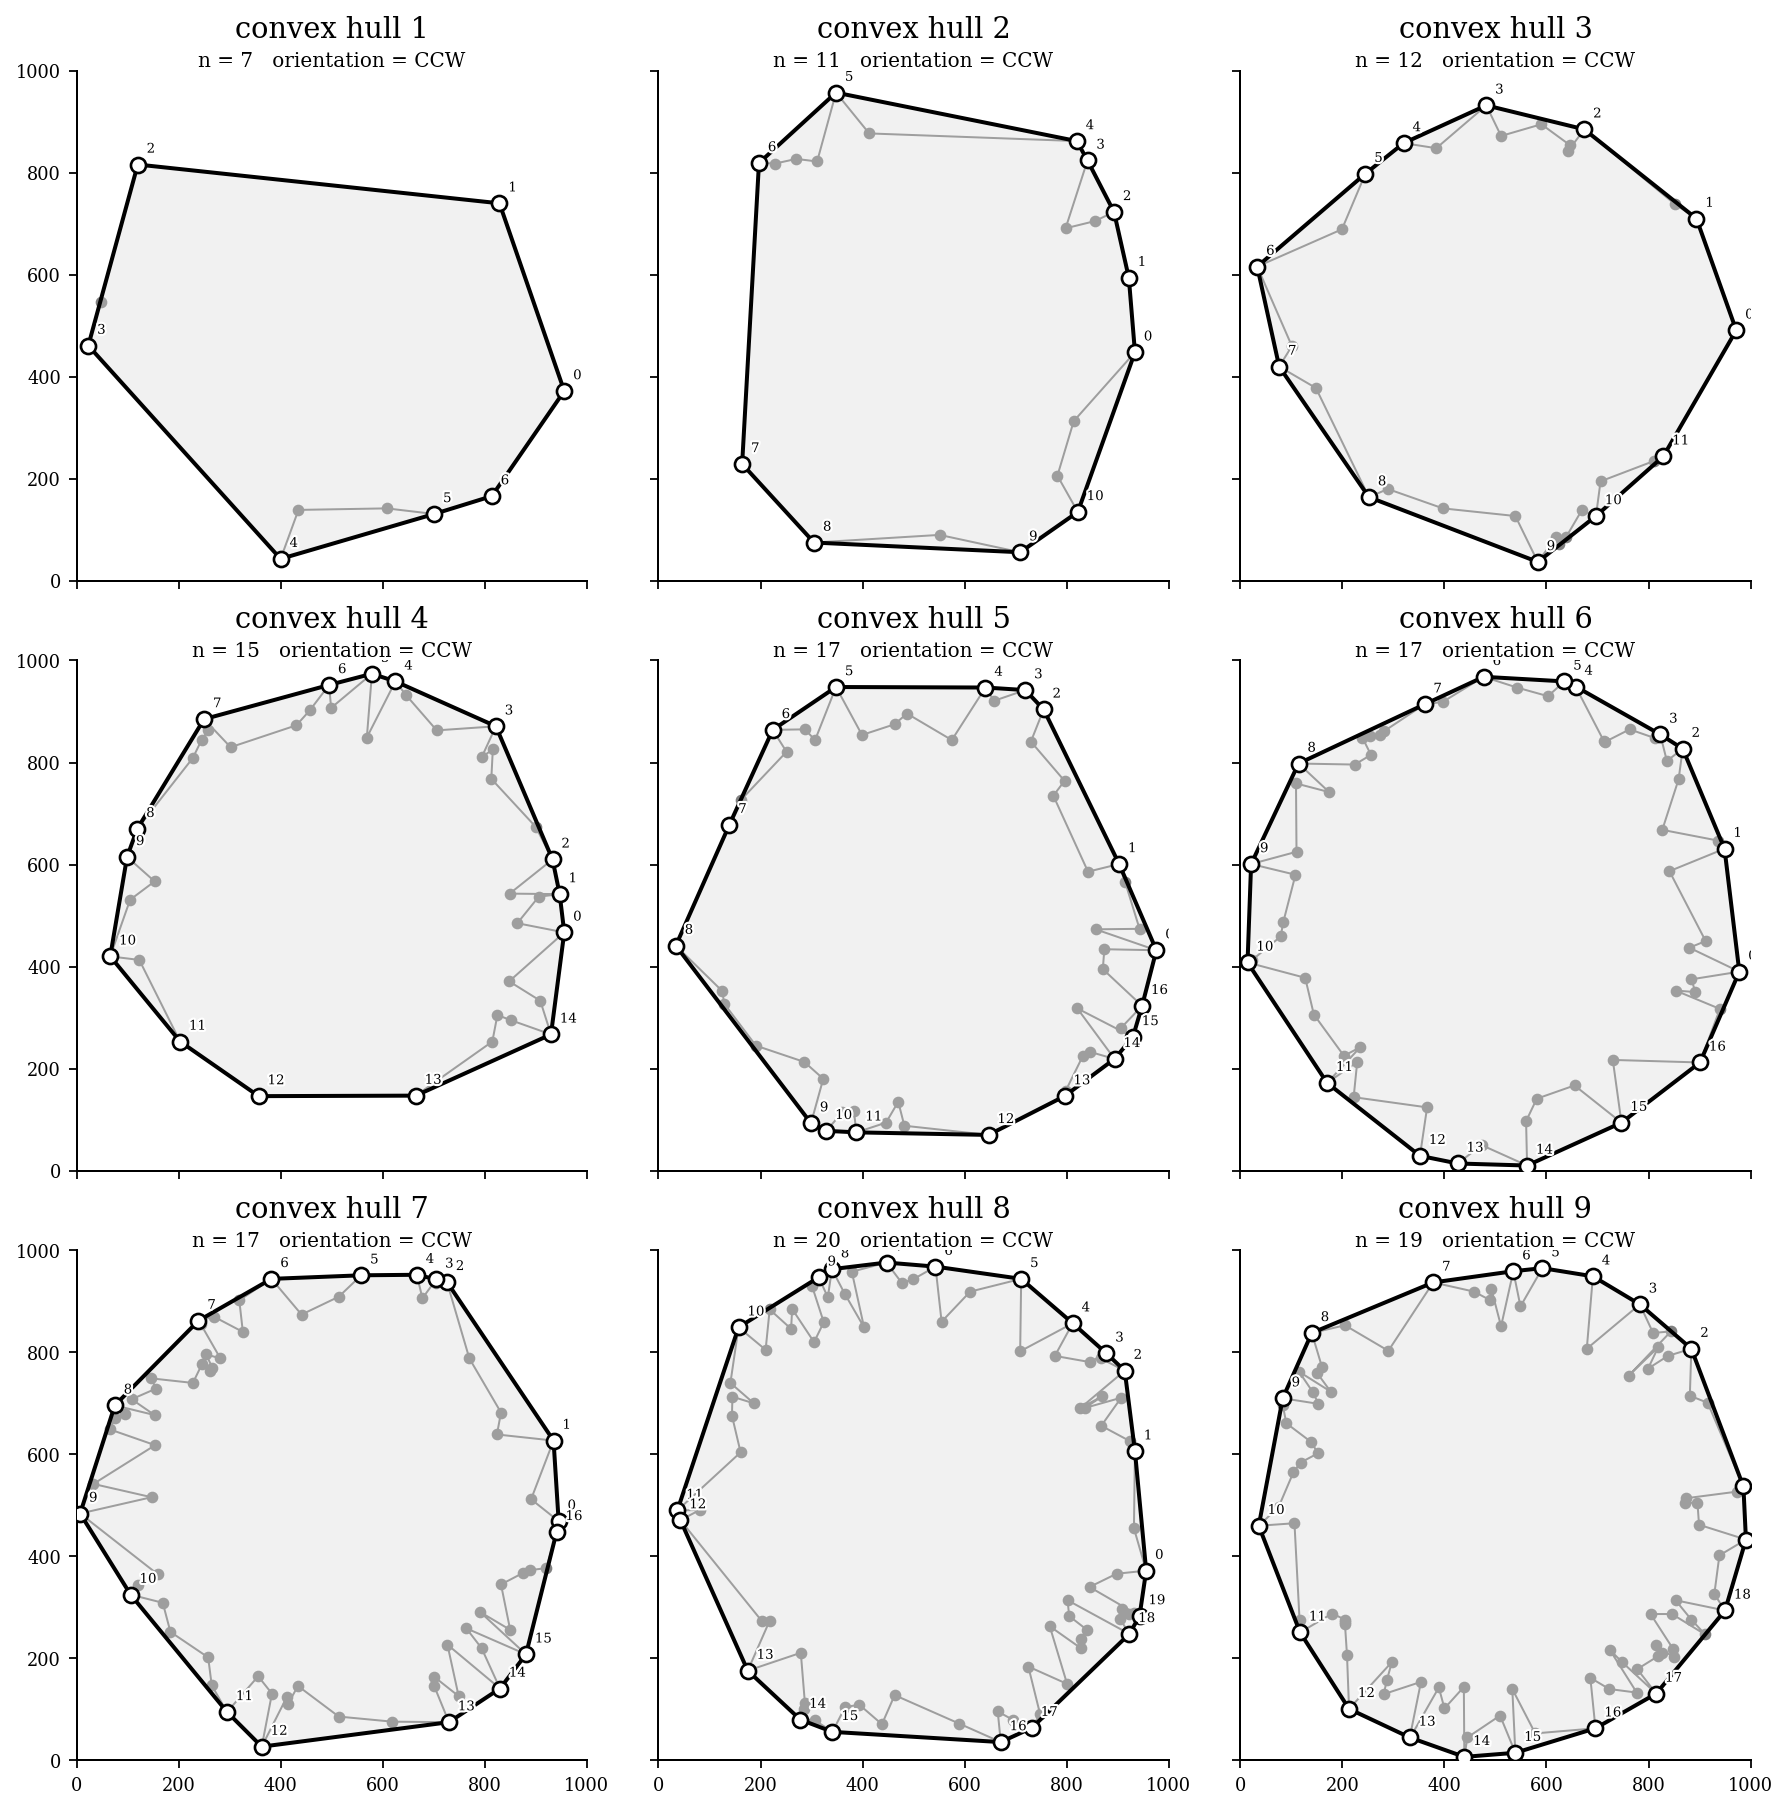
\includegraphics[width=0.95\linewidth]{Pictures/test_hulls.png}
    \caption{Convex hulls computed by Melkman’s algorithm for the polygons in Figure~\ref{fig:testpolys}, confirming correctness prior to performance analysis.}
    \label{fig:testhulls}
\end{figure}

The measured runtime and operation count were fitted to both linear and power-law models (Figure~\ref{fig:complexity}).  
The runtime grows approximately as \(T(n)\!\propto\!n^{1.28}\) (\(R^2=0.96\)), closely matching the theoretical linear trend, while operation counts exhibit an exact linear fit (\(R^2=0.99\)).  
Orientation and cross-product computations dominate total cost, whereas deque operations remain negligible.

\begin{figure}[H]
    \centering
    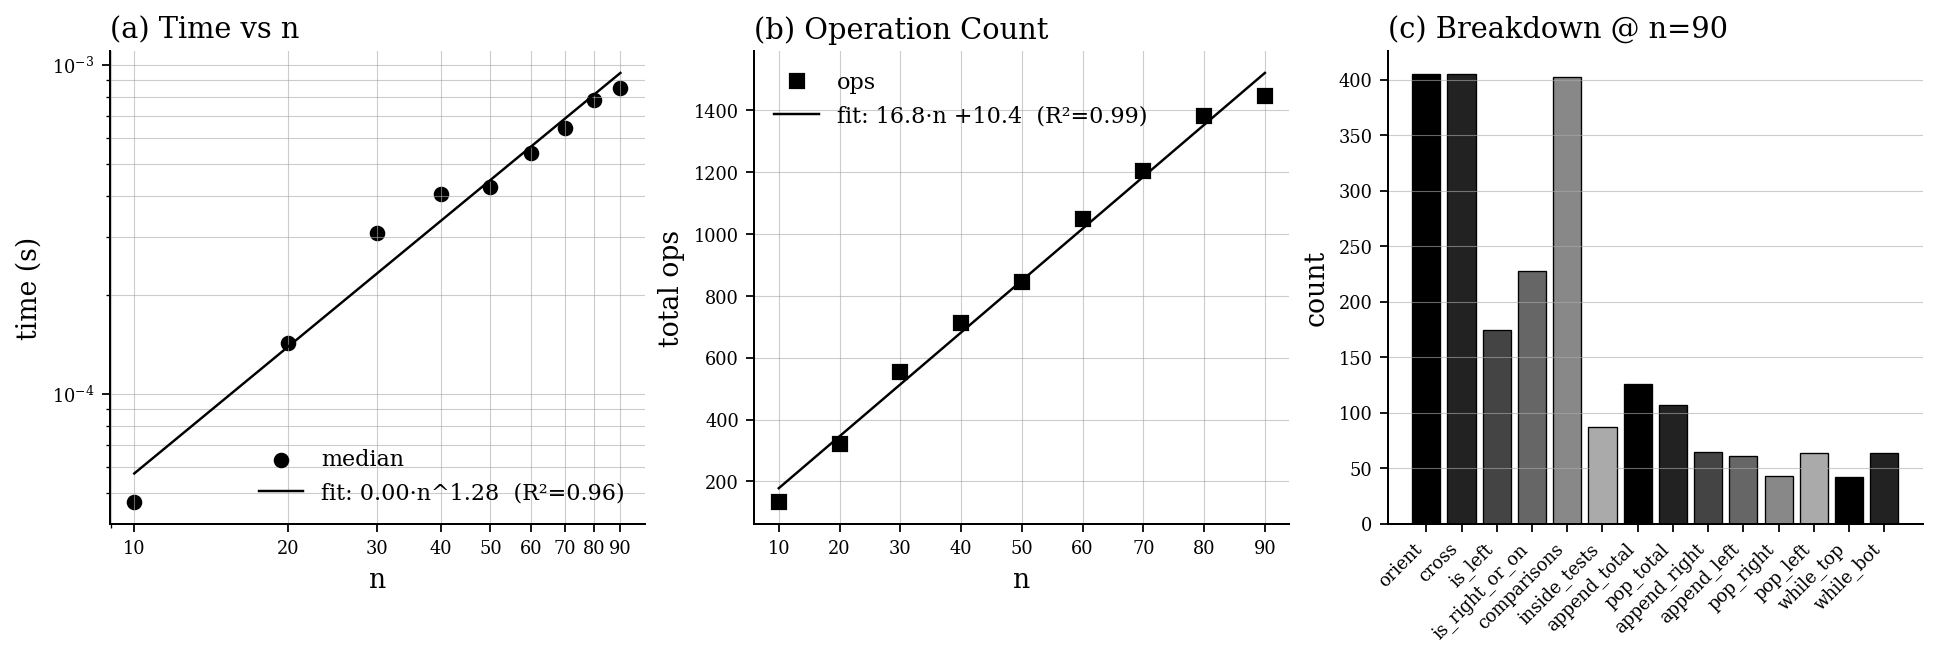
\includegraphics[width=0.95\linewidth]{Pictures/melkman_complexity.png}
    \caption{Empirical complexity analysis of Melkman’s algorithm.  
    (a) Median runtime vs.~input size $n$;  
    (b) total operation count;  
    (c) operation breakdown at $n=90$.}
    \label{fig:complexity}
\end{figure}

These empirical results confirm that the algorithm’s actual performance adheres to its theoretical design.  
Both runtime and operation growth are strictly proportional to input size, validating that Melkman’s algorithm achieves true \(\mathcal{O}(n)\) efficiency for convex hull construction on simple polygons.

% Reuse \psec and \psubsec defined in Problem 1; just reset counters here.
\setcounter{Psec}{0}
\setcounter{Psubsec}{0}

\newpage

\psec{Variant Selection and Motivation}

The variant selected in this study is the \textbf{Power Diagram} (also known as the Laguerre–Voronoi Diagram), due to its strong theoretical and practical relevance to my ongoing research on three-dimensional medical image reconstruction.  
In 3D ultrasound image segmentation and reconstruction, it is often necessary to partition the space into weighted regions according to the spatial features or importance of different points, in order to generate structurally consistent and geometrically continuous volumetric representations.  
By introducing additive weights into the distance metric, the Power Diagram allows each cell to depend not only on spatial position but also on local weighting factors, which aligns well with the inherently non-uniform distribution of anatomical structures in medical images.  
Its convexity and controllability ensure numerical stability in geometric computations, while its formulation naturally extends to three dimensions and connects seamlessly with Delaunay triangulation and regular tessellation methods.  
Therefore, the Power Diagram provides both a solid theoretical foundation and a practical geometric framework for understanding and implementing weighted spatial partitioning in 3D medical image reconstruction.

\psec{Problem Definition and Notation}

\textbf{Input.}  
A finite set of weighted sites
\[
S = \{(x_i, y_i, w_i) \mid i = 1, \dots, n\} \subset \mathbb{R}^2 \times \mathbb{R},
\]
where $(x_i, y_i)$ denotes the spatial coordinates of site $s_i$, and $w_i$ is a scalar weight determining its relative influence in the power distance metric.

\textbf{Output.}  
A per-site collection of half-planes representing the Power Diagram in implicit form.  
For each site $s_i$, its region is encoded as
\[
\mathcal{H}_i = \{(a_{ij}, b_{ij}, c_{ij}) \mid a_{ij}x + b_{ij}y \le c_{ij},\ j \neq i\},
\]
where each triple $(a_{ij}, b_{ij}, c_{ij})$ corresponds to the bisector $\phi_i \le \phi_j$.  
The explicit polygonal cell is given by
\[
V_i = \bigcap_{H \in \mathcal{H}_i} H,
\]
and the complete diagram is $\{V_i\}_{i=1}^n$.

\textbf{Power distance and cell definition.}  
For $p=(x,y)\in\mathbb{R}^2$ and site $s_i=(x_i,y_i,w_i)$, the power distance is defined as
\[
\phi_i(p) = \|p - s_i\|^2 - w_i .
\]
The \emph{power cell} associated with $s_i$ is
\[
V_i = \{p \in \mathbb{R}^2 \mid \phi_i(p) \le \phi_j(p),\ \forall j \ne i\},
\]
representing the set of all points closer (in the power sense) to $s_i$ than to any other site.

\textbf{Goal.}  
Construct the per-site half-plane sets $\{\mathcal{H}_i\}$ defining the Power Diagram, visualize the resulting cells by clipping against a finite bounding box, and analyze the algorithm’s theoretical and empirical complexity.

\textbf{Notation.}  
The main mathematical symbols used in this section are summarized in Table~\ref{tab:notation2}.

\begin{table}[H]
\centering
\caption{Notation used in Problem~2.}
\label{tab:notation2}
\renewcommand{\arraystretch}{1.1}
\begin{tabular}{p{5.0cm} p{8.3cm}}
\hline
\textbf{Symbol} & \textbf{Description} \\
\hline
$S = \{(x_i, y_i, w_i)\}_{i=1}^n$ & Set of $n$ weighted sites in $\mathbb{R}^2$ with scalar weights. \\[2pt]
$s_i = (x_i, y_i, w_i)$ & The $i$-th weighted site. \\[2pt]
$\phi_i(p) = \|p - s_i\|^2 - w_i$ & Power distance between point $p$ and site $s_i$. \\[2pt]
$V_i = \{p \mid \phi_i(p) \le \phi_j(p),\ \forall j \ne i\}$ & Power cell of $s_i$, defined by pairwise inequalities. \\[2pt]
$\mathcal{H}_i = \{(a_{ij}, b_{ij}, c_{ij}) \mid j \ne i\}$ & Set of half-plane constraints for $V_i$ with coefficients satisfying $a_{ij}x + b_{ij}y \le c_{ij}$. \\[2pt]
$(a_{ij}, b_{ij}, c_{ij})$ & Coefficients of the affine bisector between $s_i$ and $s_j$. \\[2pt]
$B = [x_{\min}, y_{\min}, x_{\max}, y_{\max}]$ & Bounding box for visualization or clipping. \\[2pt]
$H_{ij}$ & Half-plane $\{p \mid \phi_i(p) \le \phi_j(p)\}$ contributing one $(a_{ij}, b_{ij}, c_{ij})$ to $\mathcal{H}_i$. \\[2pt]
$T(n), M(n)$ & Asymptotic time and space complexities of the Power Diagram construction. \\
\hline
\end{tabular}
\end{table}

\psubsec{Data Structures}

The input is a sequential site array \(S=\{s_i\}_{i=1}^n\) with
\(s_i=(x_i,y_i,w_i)\in\mathbb{R}^2\times\mathbb{R}\).
For each ordered pair \((s_i,s_j)\), the power-bisector
\(\phi_i(p)=\phi_j(p)\) is stored as a linear half-plane
\[
a_{ij}x + b_{ij}y \le c_{ij},\qquad
a_{ij}=2(x_j-x_i),\quad
b_{ij}=2(y_j-y_i),\quad
c_{ij}=(x_j^2+y_j^2)-(x_i^2+y_i^2)+(w_i-w_j).
\]
Per site, these constraints are grouped as
\(\mathcal{H}_i=\{(a_{ij},b_{ij},c_{ij})\mid j\ne i\}\),
which encodes the cell by intersection \(V_i=\bigcap_{H\in\mathcal{H}_i}H\).
The collection \(\{\mathcal{H}_i\}_{i=1}^n\) supports later polygon
reconstruction by half-plane clipping while providing \(O(1)\) access to
each cell’s defining inequalities.

\psubsec{Algorithmic Overview}

The Power Diagram is constructed by evaluating all ordered pairs of weighted sites to derive the affine half-planes that define each cell.  
For every site \(s_i=(x_i,y_i,w_i)\), the algorithm iterates through all other sites \(s_j\ (j\neq i)\) and computes the bisector coefficients of \(\phi_i(p)\le\phi_j(p)\) in linear form:
\[
a_{ij}=2(x_j-x_i),\quad
b_{ij}=2(y_j-y_i),\quad
c_{ij}=(x_j^2+y_j^2)-(x_i^2+y_i^2)+(w_i-w_j).
\]
Each triple \((a_{ij},b_{ij},c_{ij})\) is stored in \(\mathcal{H}_i\), the constraint set representing the cell of \(s_i\).  
After all pairs are processed, the output is the collection \(\{\mathcal{H}_i\}_{i=1}^n\); convex cells can later be recovered by clipping \(\bigcap_{H\in\mathcal{H}_i}H\).

\begin{algorithm}[H]
\caption{Power Diagram Construction}
\begin{algorithmic}[1]
\Require Weighted sites \(S=\{(x_i,y_i,w_i)\}_{i=1}^n\)
\Ensure Per-site half-plane sets \(\{\mathcal{H}_i\}_{i=1}^n\)

\For{\(i=1\) to \(n\)}
    \State \(\mathcal{H}_i\gets[\,]\)
    \For{\(j=1\) to \(n\)}
        \If{\(j=i\)} \State \textbf{continue} \EndIf
        \State \(a\gets2(x_j-x_i);\ b\gets2(y_j-y_i)\)
        \State \(c\gets(x_j^2+y_j^2)-(x_i^2+y_i^2)+(w_i-w_j)\)
        \State append \((a,b,c)\) to \(\mathcal{H}_i\)
    \EndFor
\EndFor
\State \Return \(\{\mathcal{H}_i\}_{i=1}^n\)
\end{algorithmic}
\end{algorithm}

\psec{Test Case Design}

\psubsec{Special Conditions}

To ensure robustness, representative configurations are defined to capture the principal geometric and numerical challenges unique to weighted Voronoi (Power) diagrams.  
Extreme weight disparities test the algorithm’s handling of dominant sites and correctly identifying empty or vanishing cells.  
The unweighted limit (\(w_i\!\equiv\!0\)) verifies degeneration to the standard Voronoi case and correctness of affine bisector formation.  
Collinear or near-collinear sites examine numerical stability under limited angular diversity, producing elongated or semi-infinite cells.  
Negative weights evaluate the correctness of half-plane orientation when sign changes occur in \((w_i-w_j)\).  
Coincident sites with different weights confirm that the higher-weight site dominates and the lower-weight site degenerates into a zero-area region.  
Together, these scenarios define the space of valid yet challenging inputs against which the subsequent Power Diagram cases are systematically designed.

\psubsec{Case Design}

\textbf{Case 1: Unweighted Baseline with Collinear Strip Degeneracy.}  
All weights are set to \(w_i\!\equiv\!0\) to reproduce the classical Voronoi limit while stressing affine bisectors under extended collinearity.  
A subset of sites is arranged collinearly to generate near-parallel bisectors and elongated cells, while the remaining sites are positioned off the line to preserve a two-dimensional configuration and avoid 1D collapse.  
This setting verifies correct degeneration to the unweighted Voronoi behavior, evaluates the numerical stability of half-plane generation and polygon recovery under limited angular diversity, and confirms that boundedness or unboundedness arises purely from geometry rather than numerical artifacts.

\textbf{Case 2: Extreme Weight Dominance with a Negative-Weight Outlier.}  
This case investigates two weight-dependent extremes absent in the classical Voronoi model: strong positive dominance and negative-weight behavior.  
A single site with a significantly larger weight enforces cell expansion and neighbor suppression, while a negative-weight site tests sign-sensitive bisector orientation.  
Moderate, asymmetrically distributed weights prevent coefficient cancellation and maintain numerical generality.  
The configuration validates correct handling of empty cells under dominance, preserves convex linear partitions across large \(|w_i-w_j|\), and demonstrates robustness of affine bisector construction in mixed positive–negative weighting regimes.

\textbf{Case 3: Coincident Sites with Mild Weights and a Weak Collinear Triplet.}  
This case examines power-based dominance at identical coordinates and local collinearity robustness.  
Pairs of coincident sites differ slightly in weight, ensuring that the higher-weight site fully dominates while the lower-weight site collapses into a zero-area cell.  
Other sites exhibit mild weight variation, with a short nearly collinear triplet included to test local geometric stability without inducing global degeneracy.  
The configuration confirms correct priority handling at coincident locations, stable bisector formation near near-collinear alignments, and preservation of well-defined convex topology without spurious empty or overlapping regions.

\psubsec{Visual Summary and Case Coverage}

\begin{figure}[H]
    \centering
    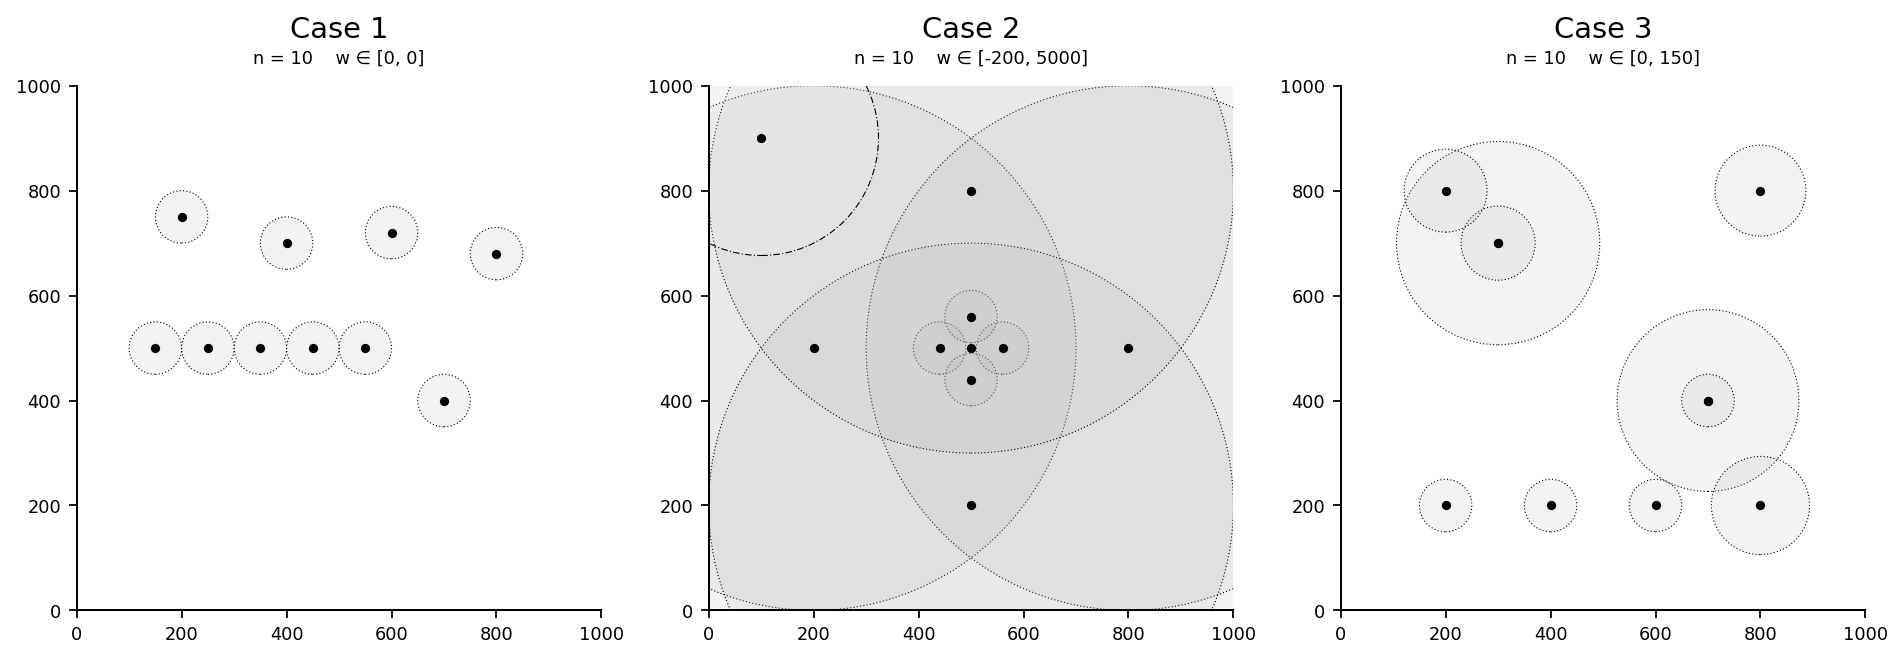
\includegraphics[width=0.95\linewidth]{Pictures/sites_cases.png}
    \caption{Representative site configurations for testing the Power Diagram algorithm. 
    Case~1: unweighted baseline with collinear strip; 
    Case~2: extreme positive weight dominance with a negative-weight outlier; 
    Case~3: coincident-site pairs with mild weights and weak collinearity.}
\end{figure}

The three designed configurations collectively capture the major geometric and weighted degeneracies encountered in Power Diagram construction.  
Case~1 verifies correct degeneration to the classical Voronoi form and stability of affine bisectors under extended collinearity.  
Case~2 evaluates robustness across large weight disparities and mixed signs, confirming dominance-induced suppression and correctness of bisector orientation.  
Case~3 tests coincident-site dominance and local collinearity, validating zero-area detection and numerical stability in typical weighted settings.  
Together, these cases provide a compact yet comprehensive validation of half-plane generation, empty-cell handling, and convex polygon recovery, demonstrating that the algorithm remains consistent and stable across all representative input regimes.

\psec{Visualization and Results Analysis}

\begin{figure}[H]
    \centering
    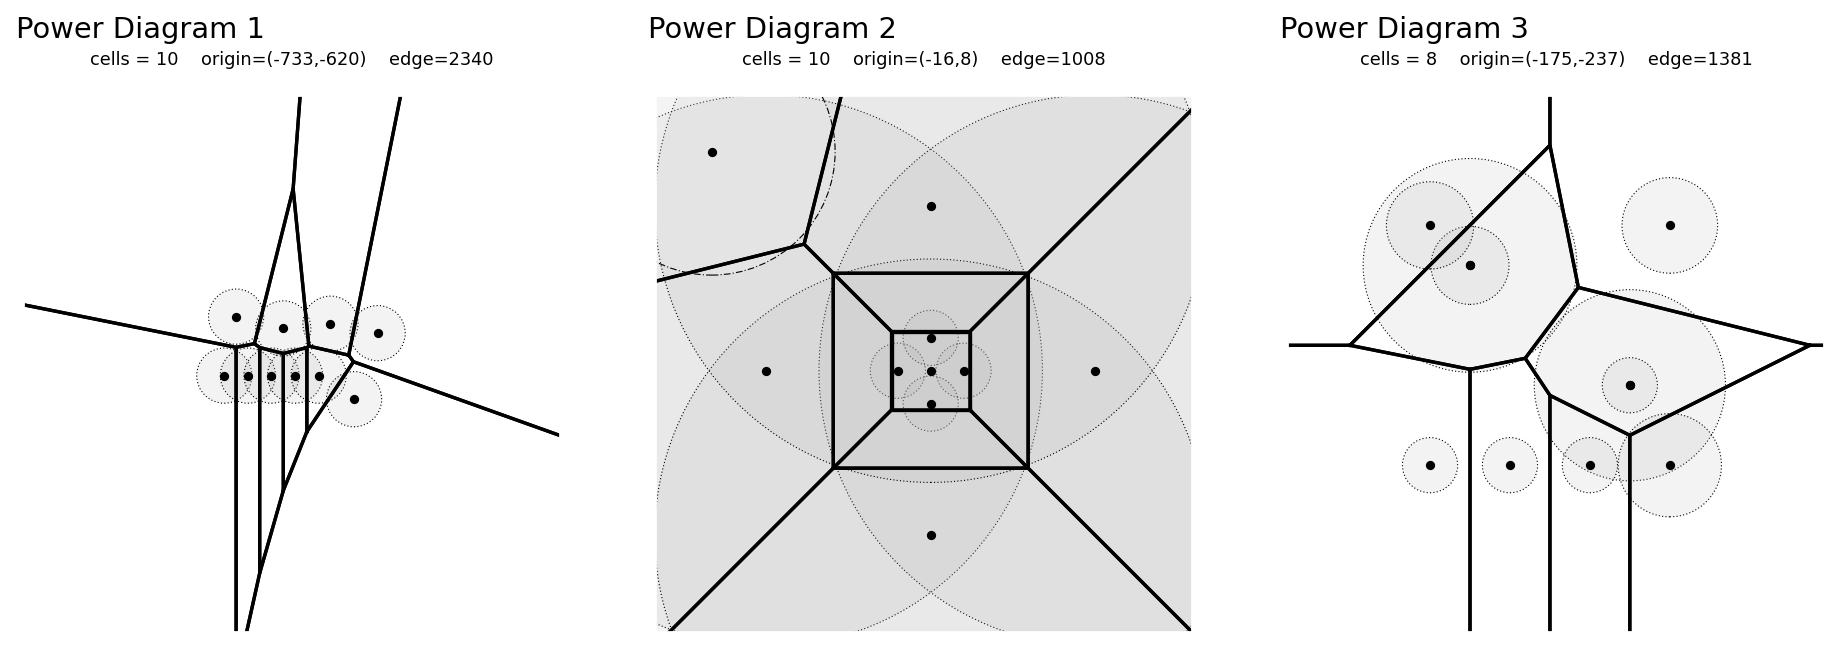
\includegraphics[width=0.95\linewidth]{Pictures/power_diagram.png}
    \caption{Power Diagrams generated for the three designed cases. 
    Black dots indicate weighted sites, thick lines denote computed power cells, and dashed circles represent visualized power radii.}
    \label{fig:power_diagrams}
\end{figure}

The visualization results confirm the geometric and numerical correctness of the Power Diagram construction across all tested conditions.  
In the unweighted case, the algorithm reproduces the standard Voronoi diagram with stable bisector formation under extended collinearity.  
Under extreme weight disparity, dominant sites expand as expected while weaker or negatively weighted sites contract or vanish, verifying consistent handling of mixed-sign weights and empty-cell detection.  
For coincident sites and weak collinearity, the algorithm correctly assigns dominance to higher-weight sites and maintains stable affine bisectors without topological artifacts.  
Across all cases, the resulting partitions remain convex, non-overlapping, and numerically well-conditioned, demonstrating robustness and correctness of the implemented Power Diagram construction Algorithm.

\psec{Complexity Analysis}

\psubsec{Theoretical}

The Power Diagram construction evaluates all ordered pairs of weighted sites to compute affine half-plane coefficients defining pairwise bisectors.  
Given \(n\) sites \(S=\{(x_i,y_i,w_i)\}_{i=1}^n\), each site \(s_i\) compares with every other \(s_j\ (j\ne i)\), producing \(n(n-1)\) half-plane constraints in total.  
Each computation involves a fixed number of arithmetic operations,
\[
a_{ij}=2(x_j-x_i),\quad b_{ij}=2(y_j-y_i),\quad c_{ij}=(x_j^2+y_j^2)-(x_i^2+y_i^2)+(w_i-w_j),
\]
executed in constant time.  
No iterative refinement or sorting is required, so the total cost grows quadratically:
\[
T(n)=\Theta(n^2).
\]
Storage is similarly dominated by the \(n(n-1)\) half-plane records across all sites, yielding
\[
M(n)=\Theta(n^2).
\]
Hence, both time and space complexities of the Power Diagram construction scale quadratically with the number of sites.

\psubsec{Empirical}

To verify the theoretical $\Theta(n^2)$ time and space complexity of the Power Diagram construction, an empirical study was conducted to observe how runtime, operation count, and memory usage scale with problem size.  
Theoretically, if each ordered site pair contributes a constant computational cost for half-plane evaluation, both time and space requirements should increase quadratically with the number of sites $n$.  
Accordingly, runtime $T(n)$ and memory cost $M(n)$ were measured as functions of $n$ over progressively enlarged site sets, where each site configuration represents an independent problem instance.

The first round of experiments used site counts from $n=5$ to $45$, as shown in Figures~\ref{fig:test_sites1}–\ref{fig:test_pd1}.  
Each dataset was randomly generated with variable coordinates and weights to ensure statistical diversity while preserving consistent geometric density.  
Measured results in Figure~\ref{fig:power_complexity1} exhibit clearly quadratic growth in operation and memory counts ($R^2\!=\!1.00$), while the runtime curve showed minor deviation and partial alignment with an $n\log n$ trend.  
This deviation arises from interpreter-level overhead and limited sample size, as the small input range causes constant factors to dominate the measured timing.

\begin{figure}[H]
    \centering
    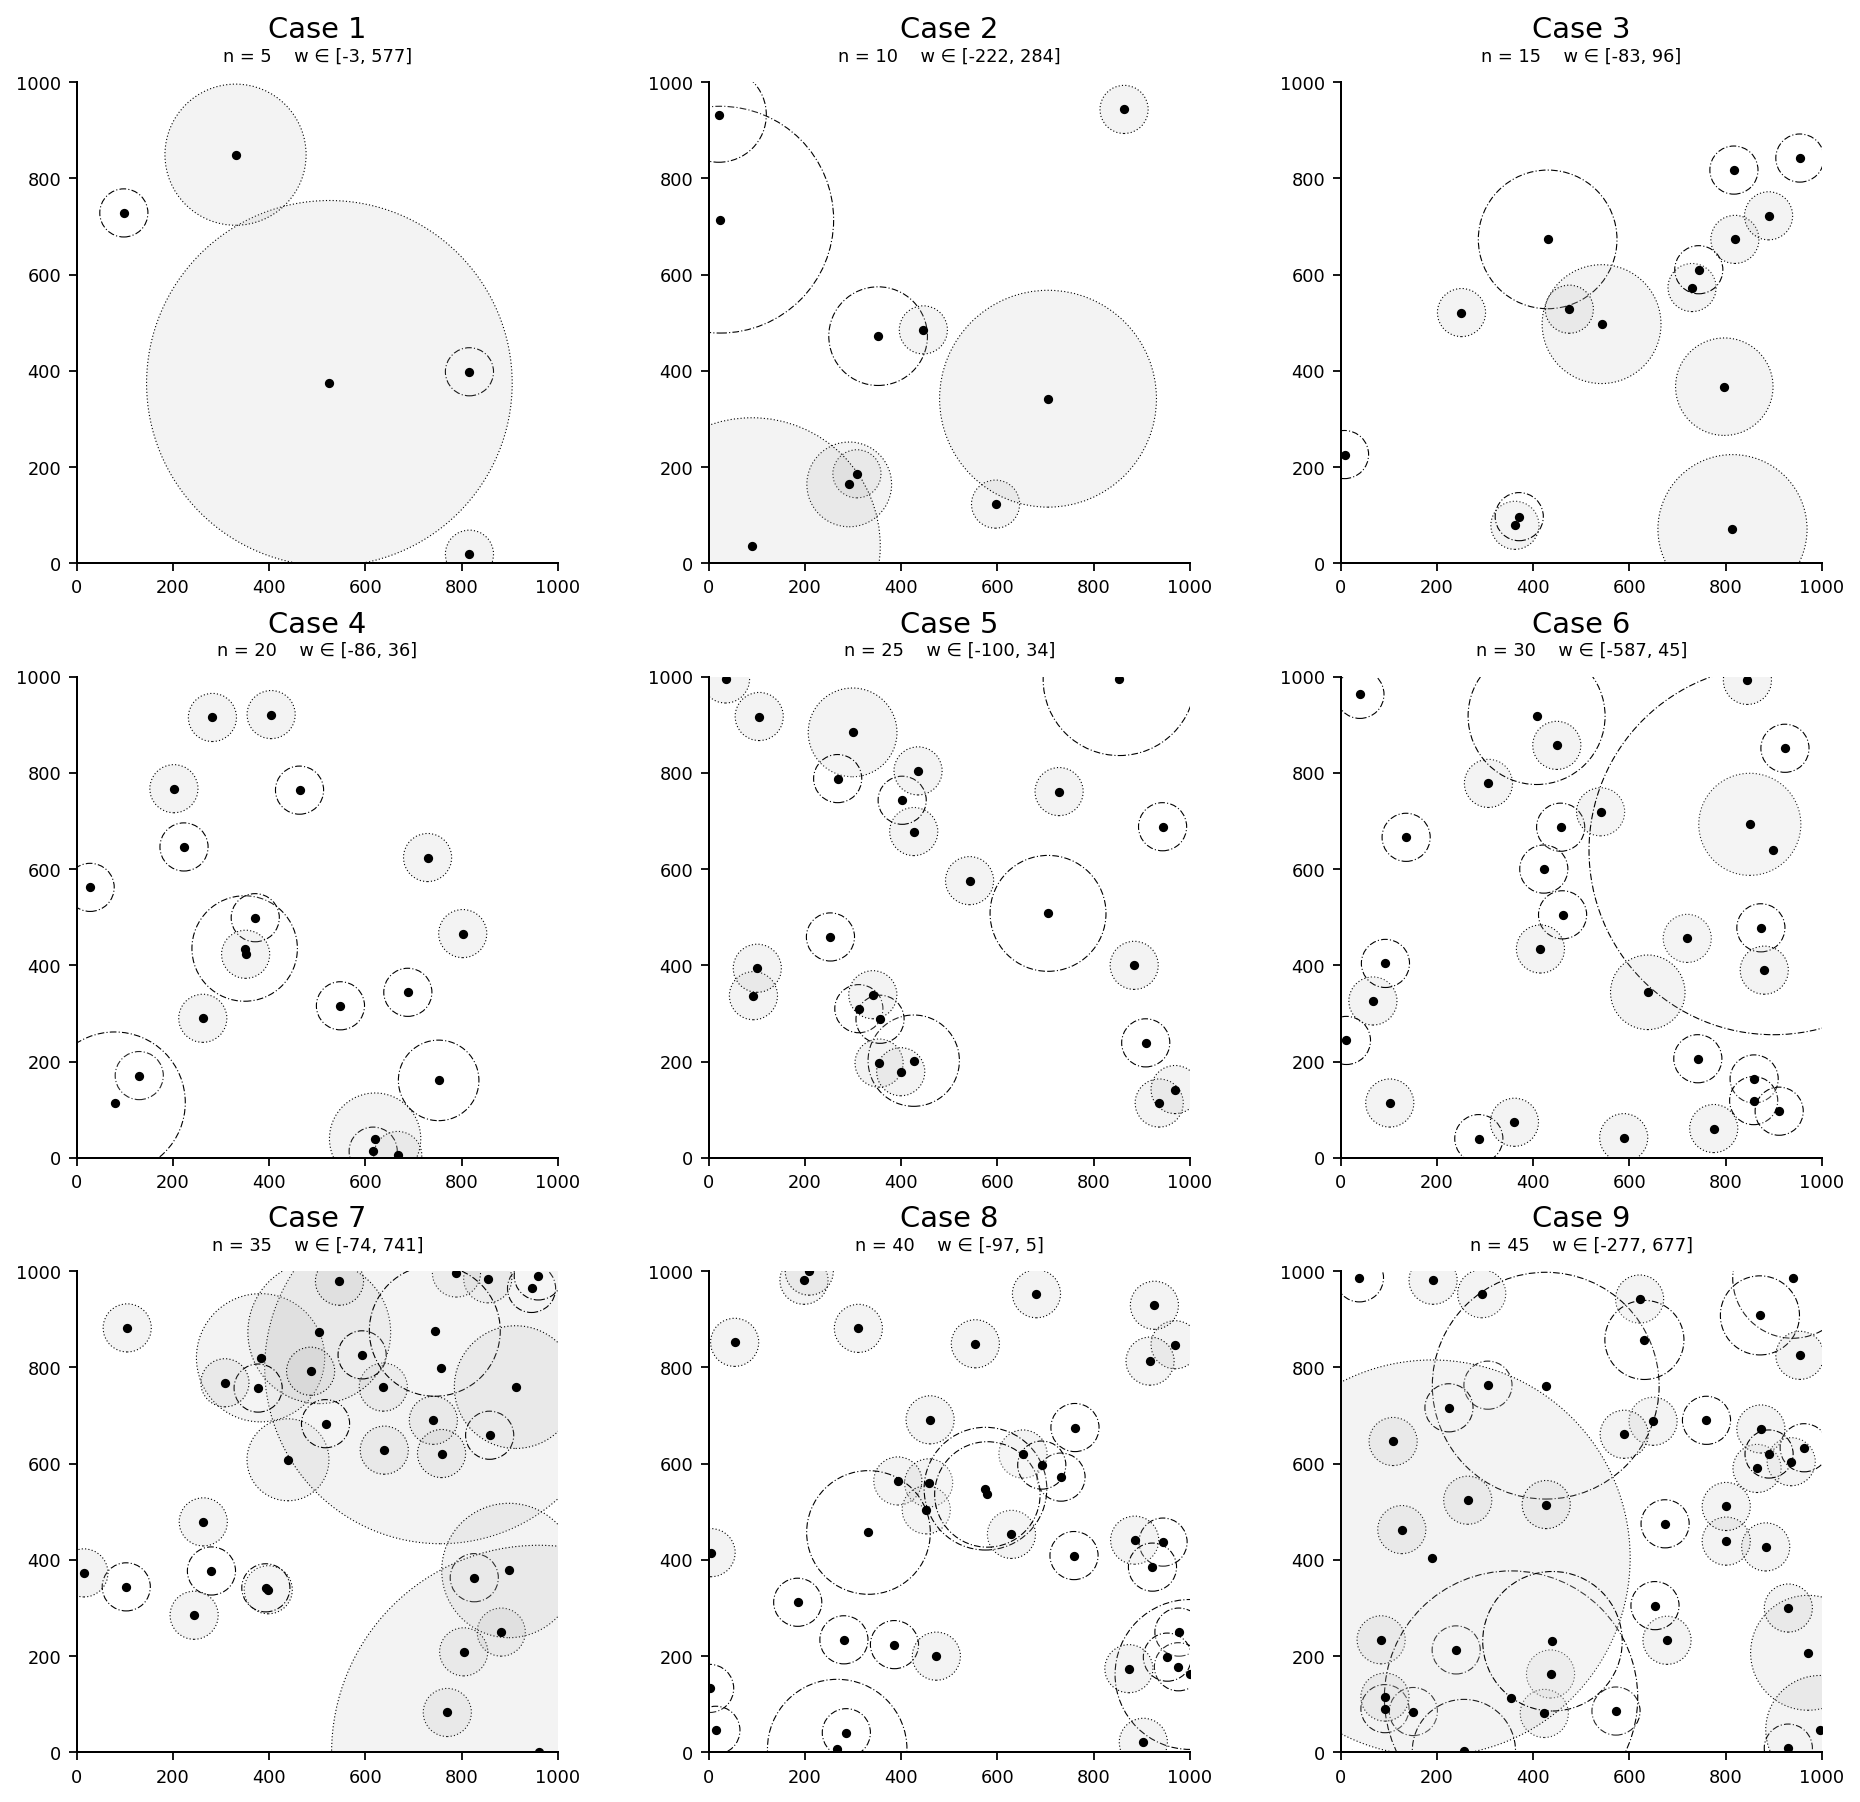
\includegraphics[width=0.95\linewidth]{Pictures/test_sites1.png}
    \caption{Generated weighted-site configurations ($n=5$–$45$) and their corresponding Power Diagrams in Figure~\ref{fig:test_pd1}.}
    \label{fig:test_sites1}
\end{figure}

\begin{figure}[H]
    \centering
    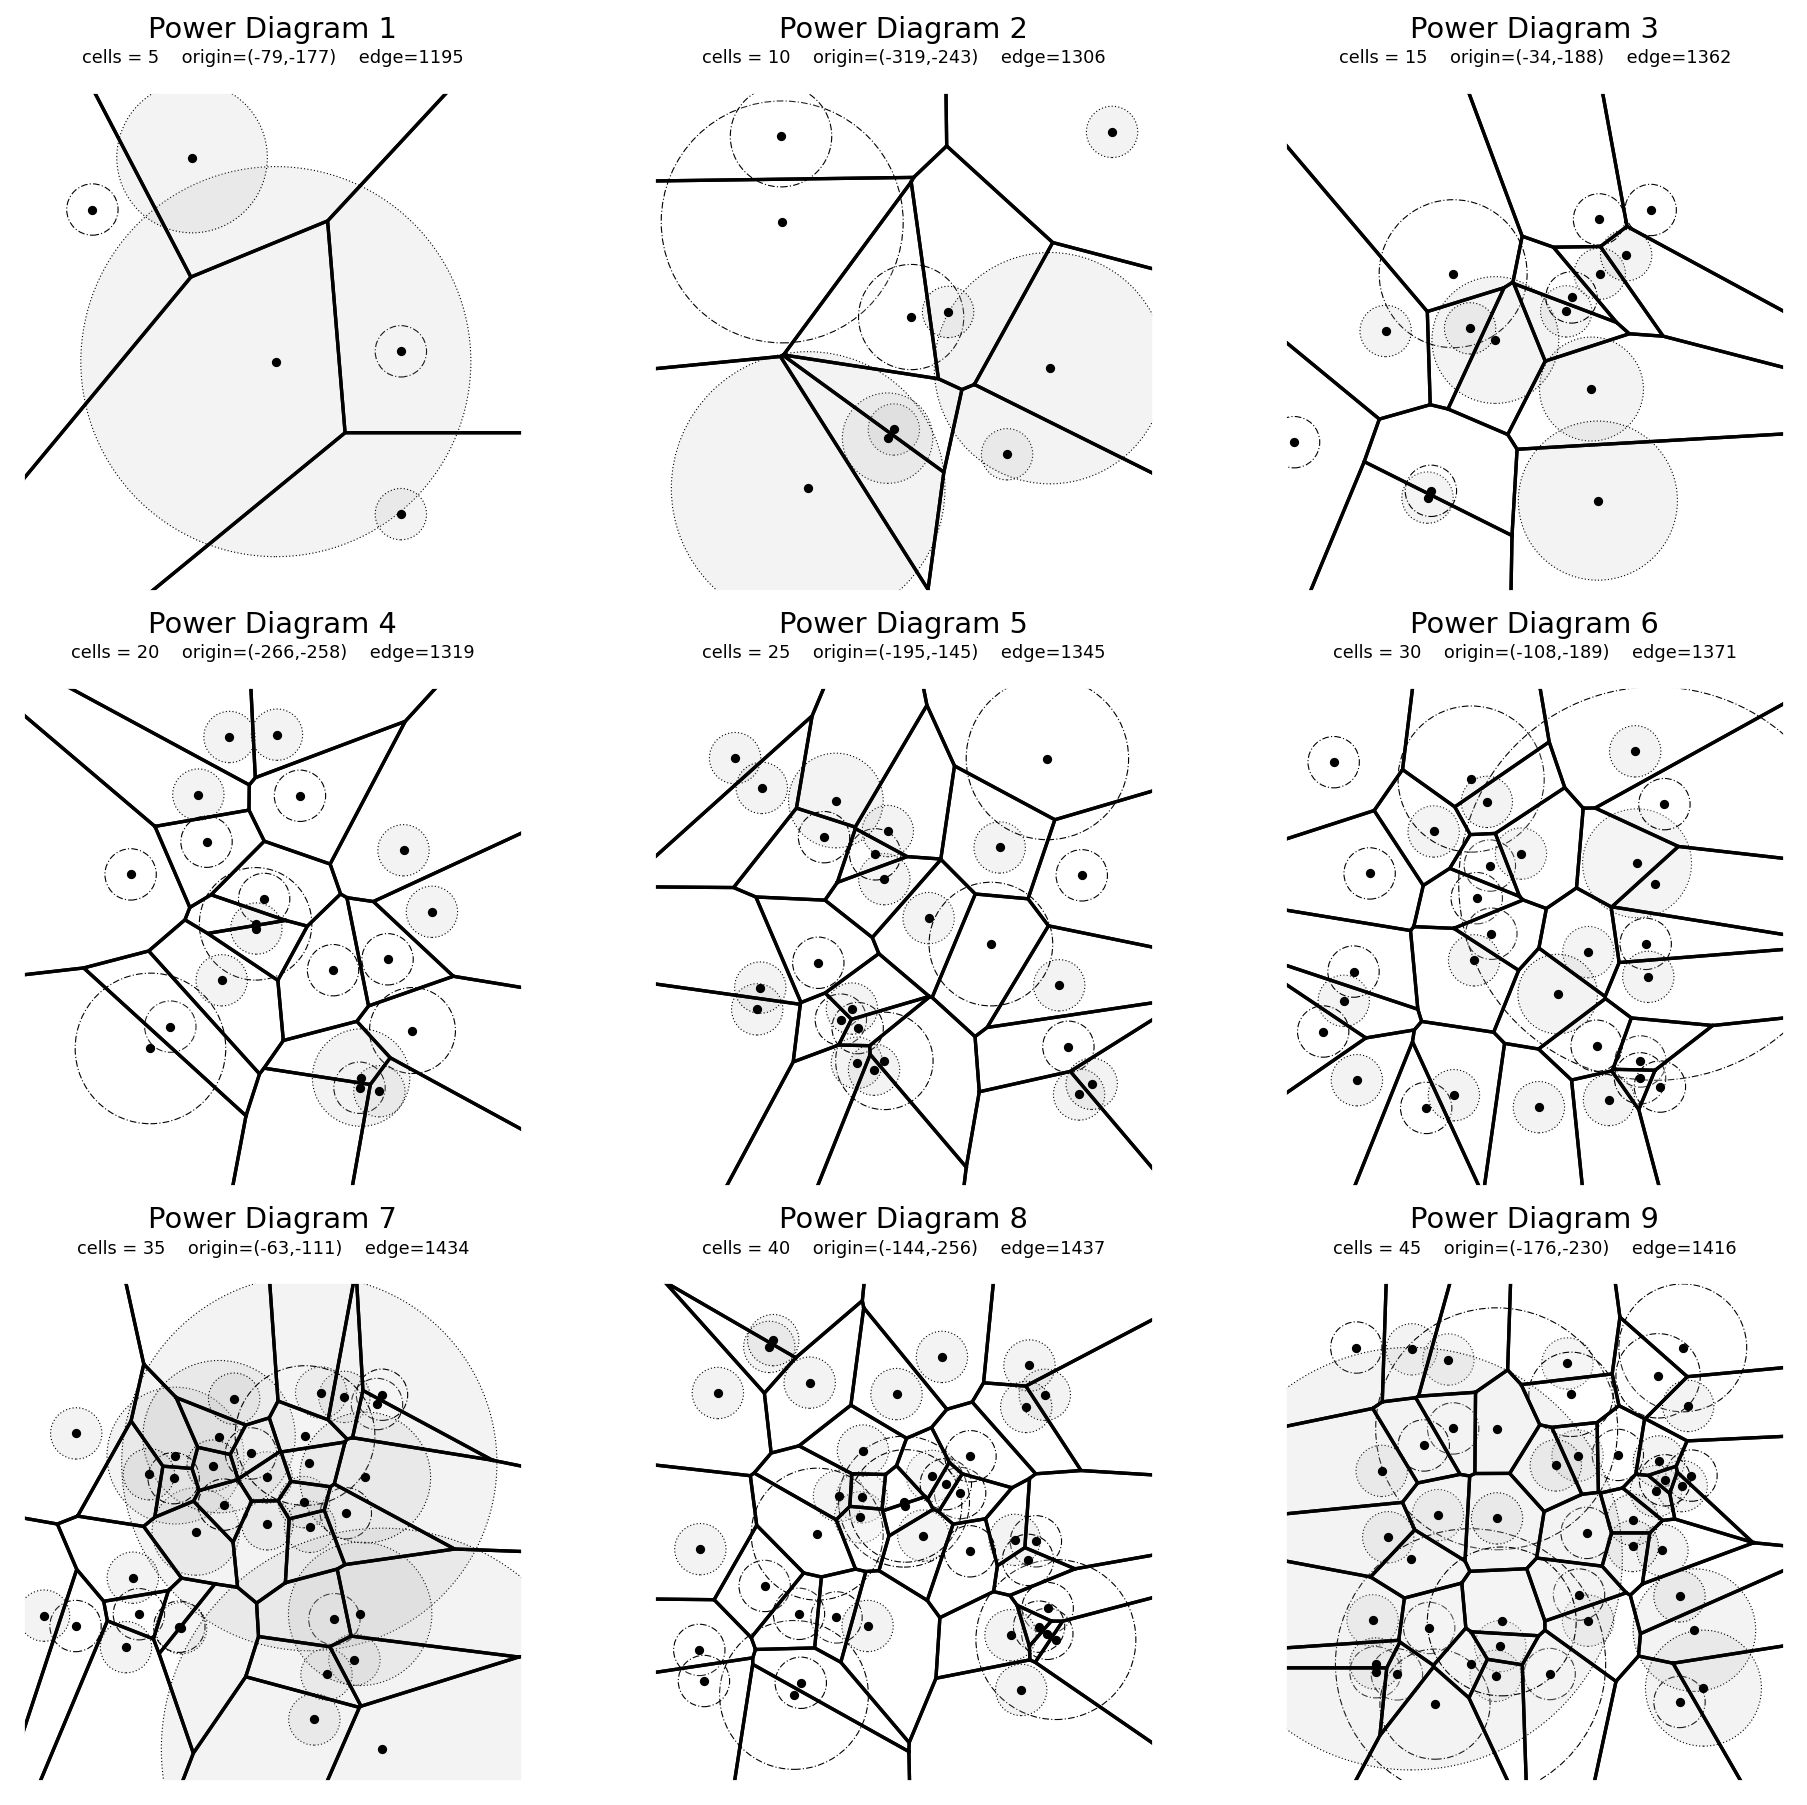
\includegraphics[width=0.95\linewidth]{Pictures/test_pd1.png}
    \caption{Power Diagram results for the first experiment, verifying correctness under small-to-medium input scales.}
    \label{fig:test_pd1}
\end{figure}

\begin{figure}[H]
    \centering
    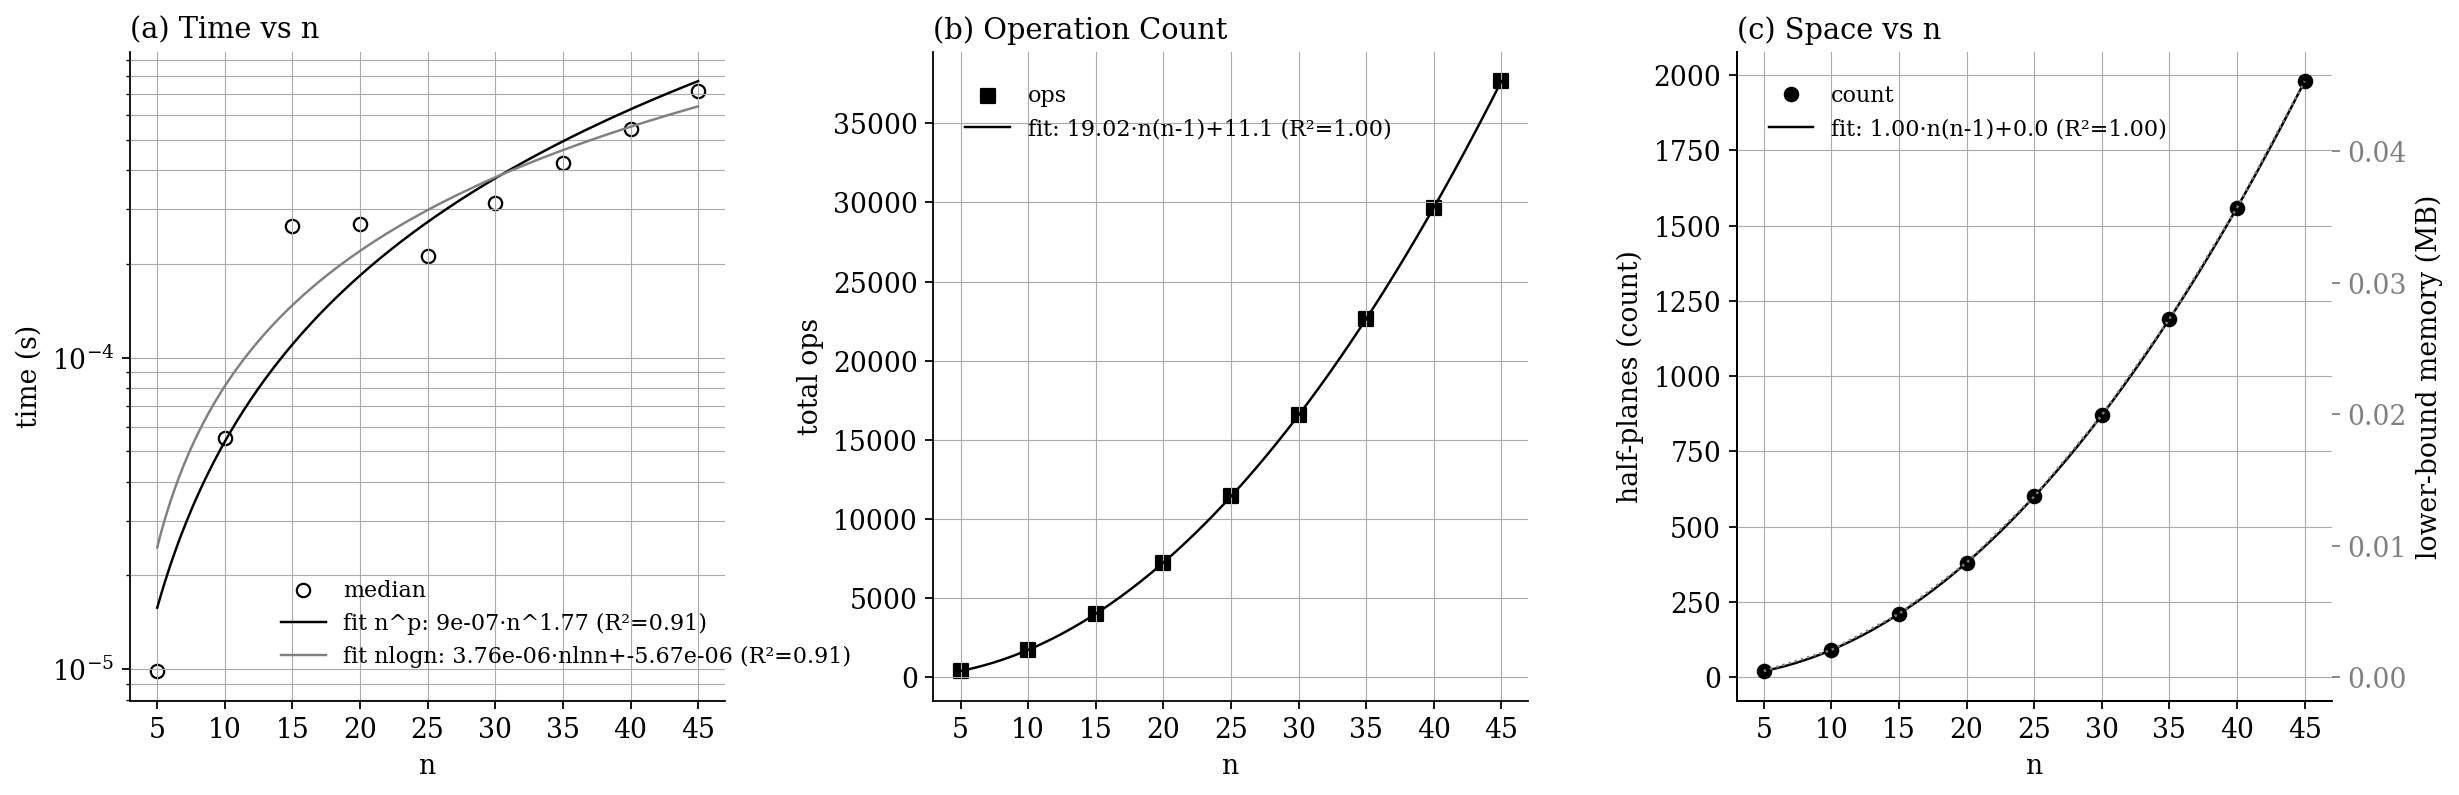
\includegraphics[width=0.95\linewidth]{Pictures/power_complexity1.png}
    \caption{Empirical complexity results for the first experiment ($n=5$–$45$). 
    (a) Runtime vs.~$n$, with $n^2$ and $n\log n$ fits; 
    (b) operation count ($R^2\!=\!1.00$); 
    (c) space usage showing perfect quadratic growth.}
    \label{fig:power_complexity1}
\end{figure}

To reduce timing noise and expose the asymptotic regime, a second experiment extended the input scale to $n=240$, as shown in Figures~\ref{fig:test_sites2}–\ref{fig:test_pd2}.  
Larger datasets eliminated low-level overhead effects, producing smooth and consistent quadratic fits across all metrics.  
As reported in Figure~\ref{fig:power_complexity2}, the runtime follows $T(n)\!\propto\!n^{1.99}$ ($R^2\!=\!1.00$), operation counts fit $19.0\,n(n-1)+44.8$ ($R^2\!=\!1.00$), and space growth remains perfectly quadratic with respect to stored half-planes.

\begin{figure}[H]
    \centering
    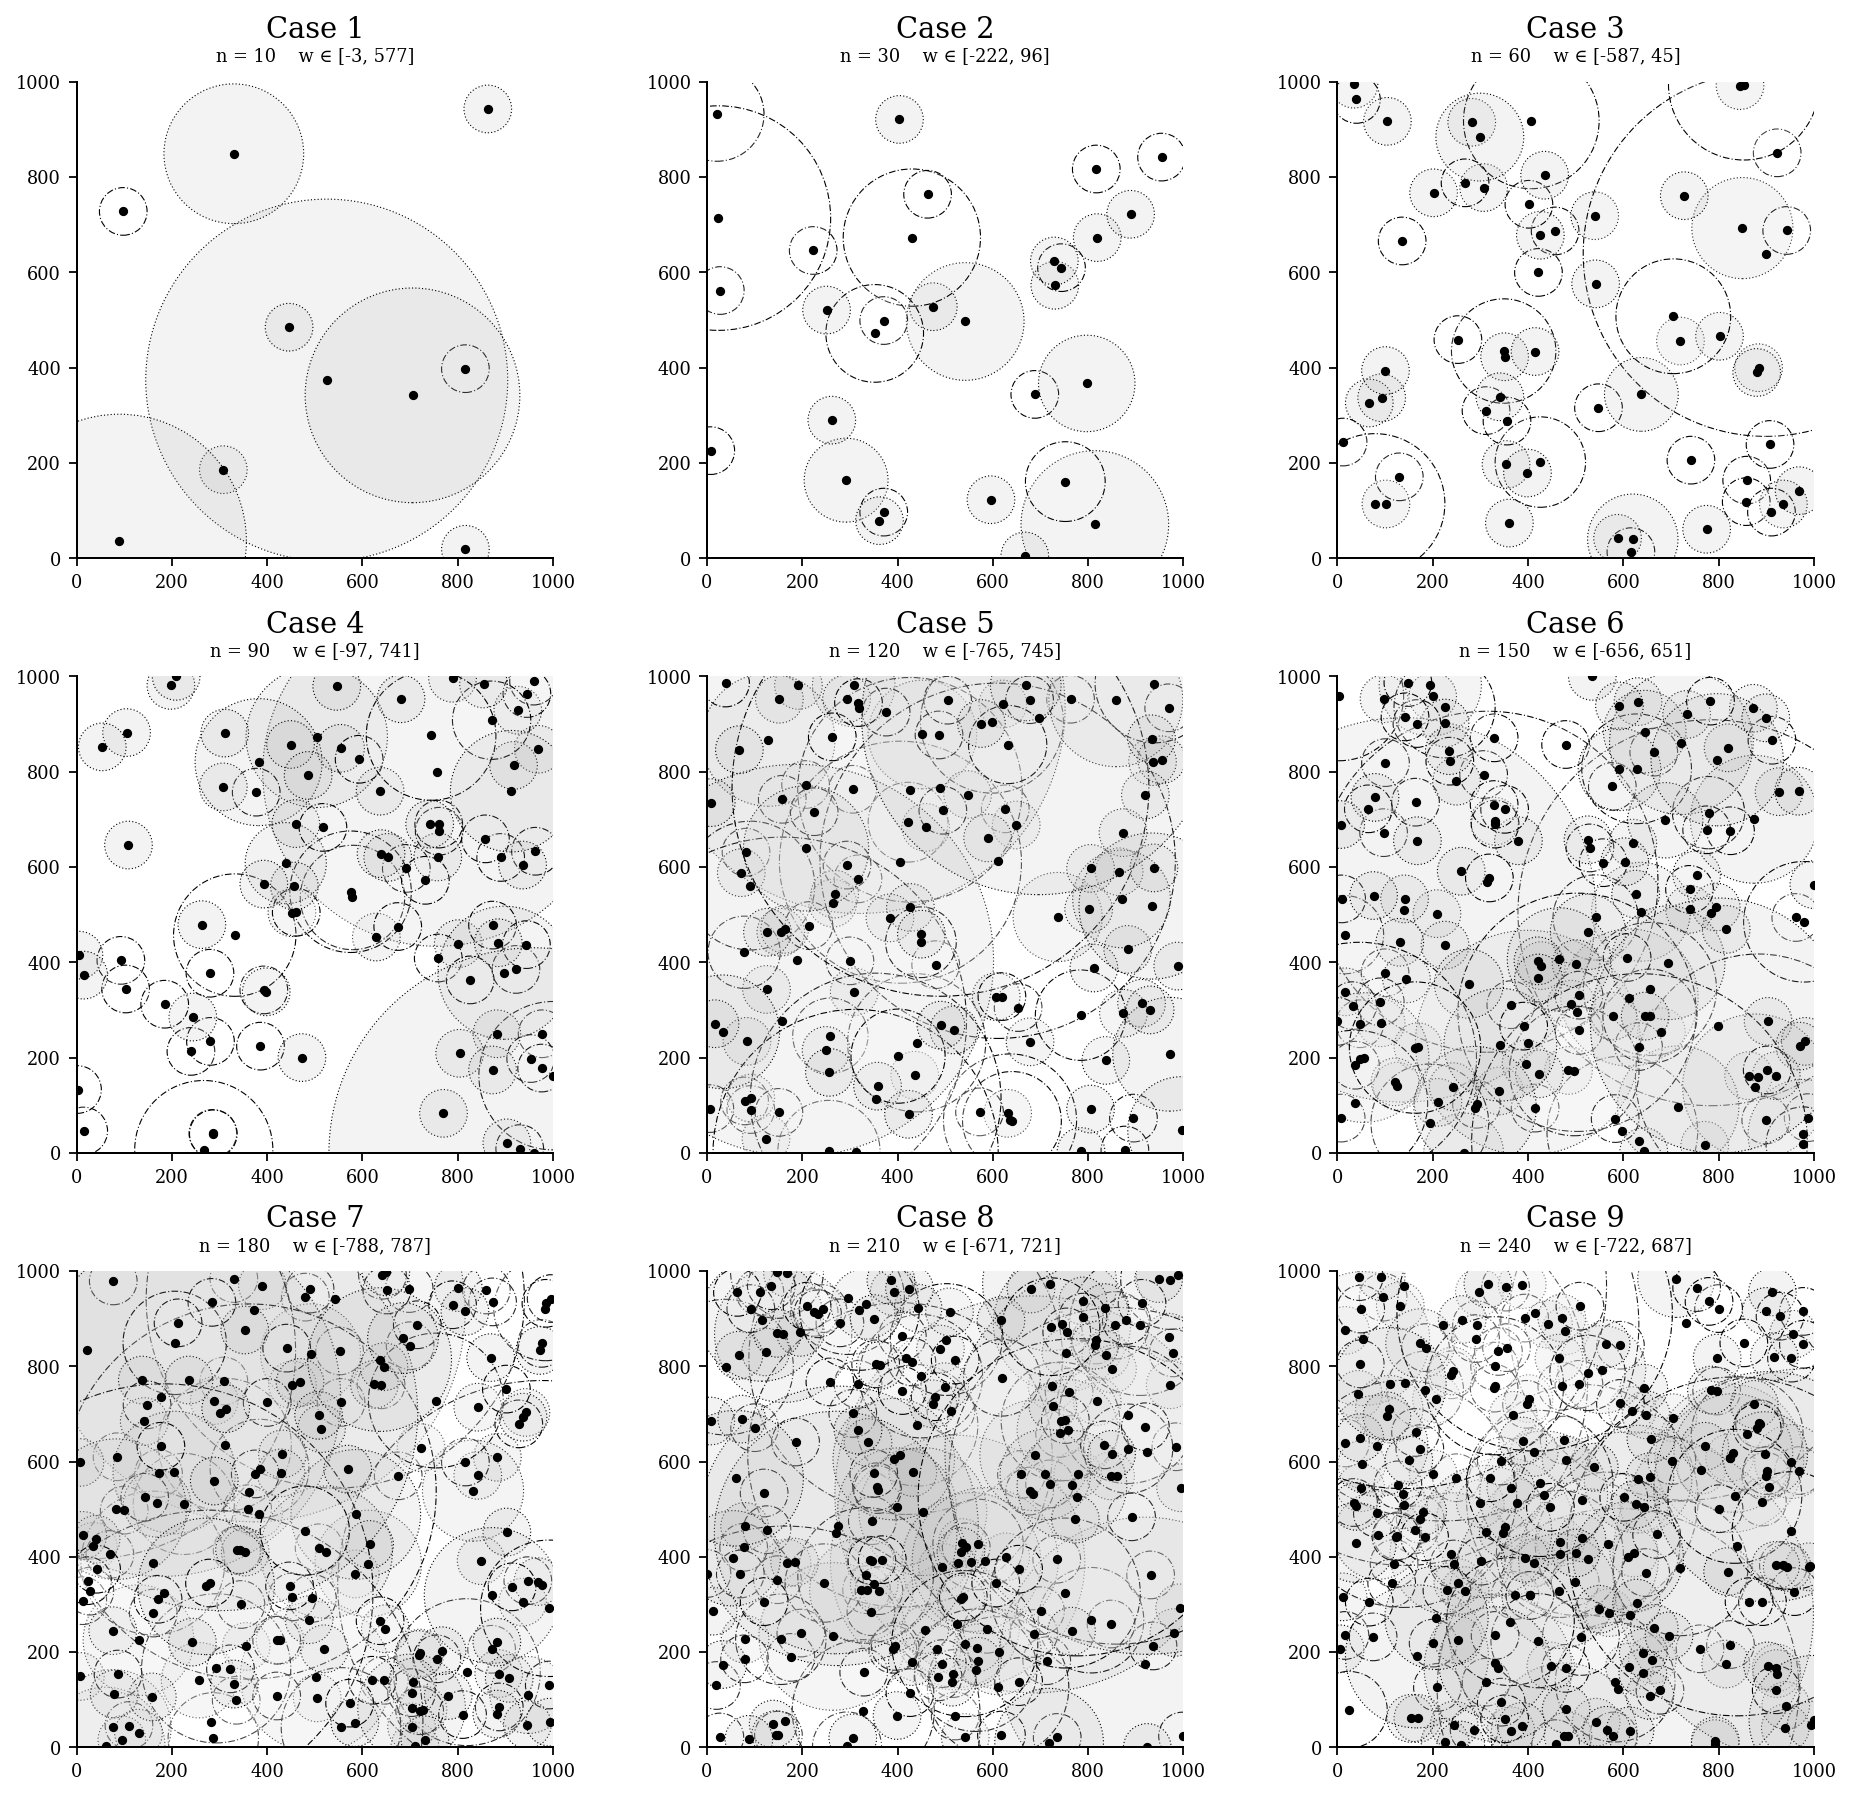
\includegraphics[width=0.95\linewidth]{Pictures/test_sites2.png}
    \caption{Weighted-site configurations for the extended experiment ($n=10$–$240$).}
    \label{fig:test_sites2}
\end{figure}

\begin{figure}[H]
    \centering
    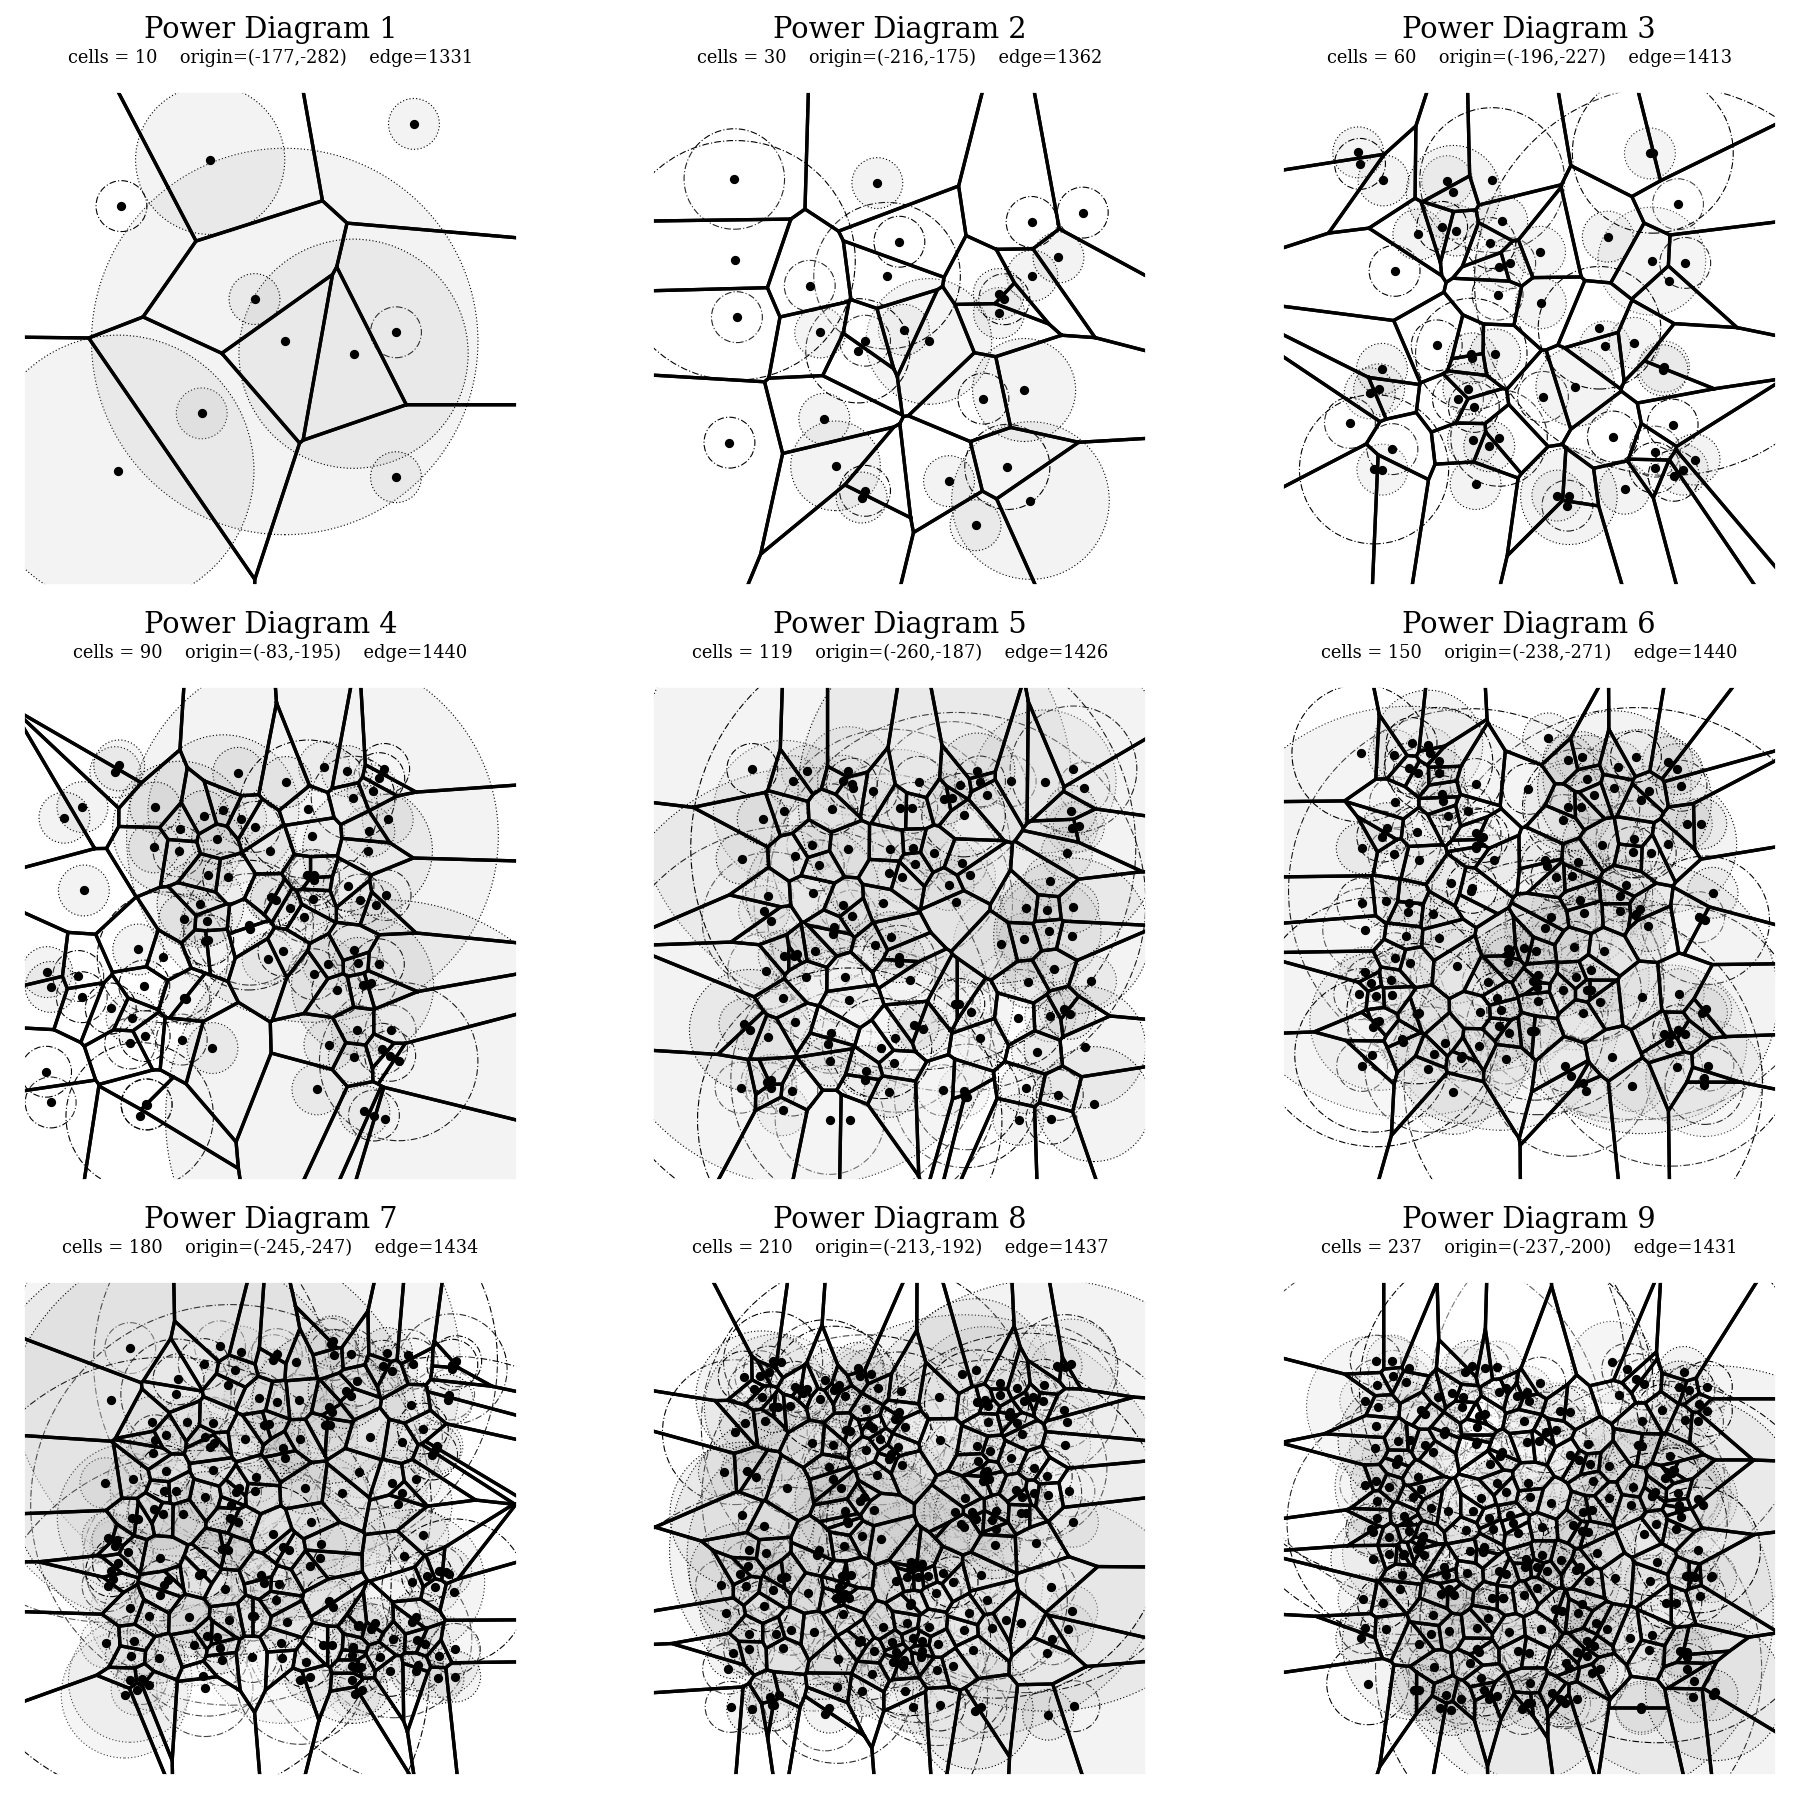
\includegraphics[width=0.95\linewidth]{Pictures/test_pd2.png}
    \caption{Power Diagrams corresponding to Figure~\ref{fig:test_sites2}, demonstrating stability and correctness at large scales.}
    \label{fig:test_pd2}
\end{figure}

\begin{figure}[H]
    \centering
    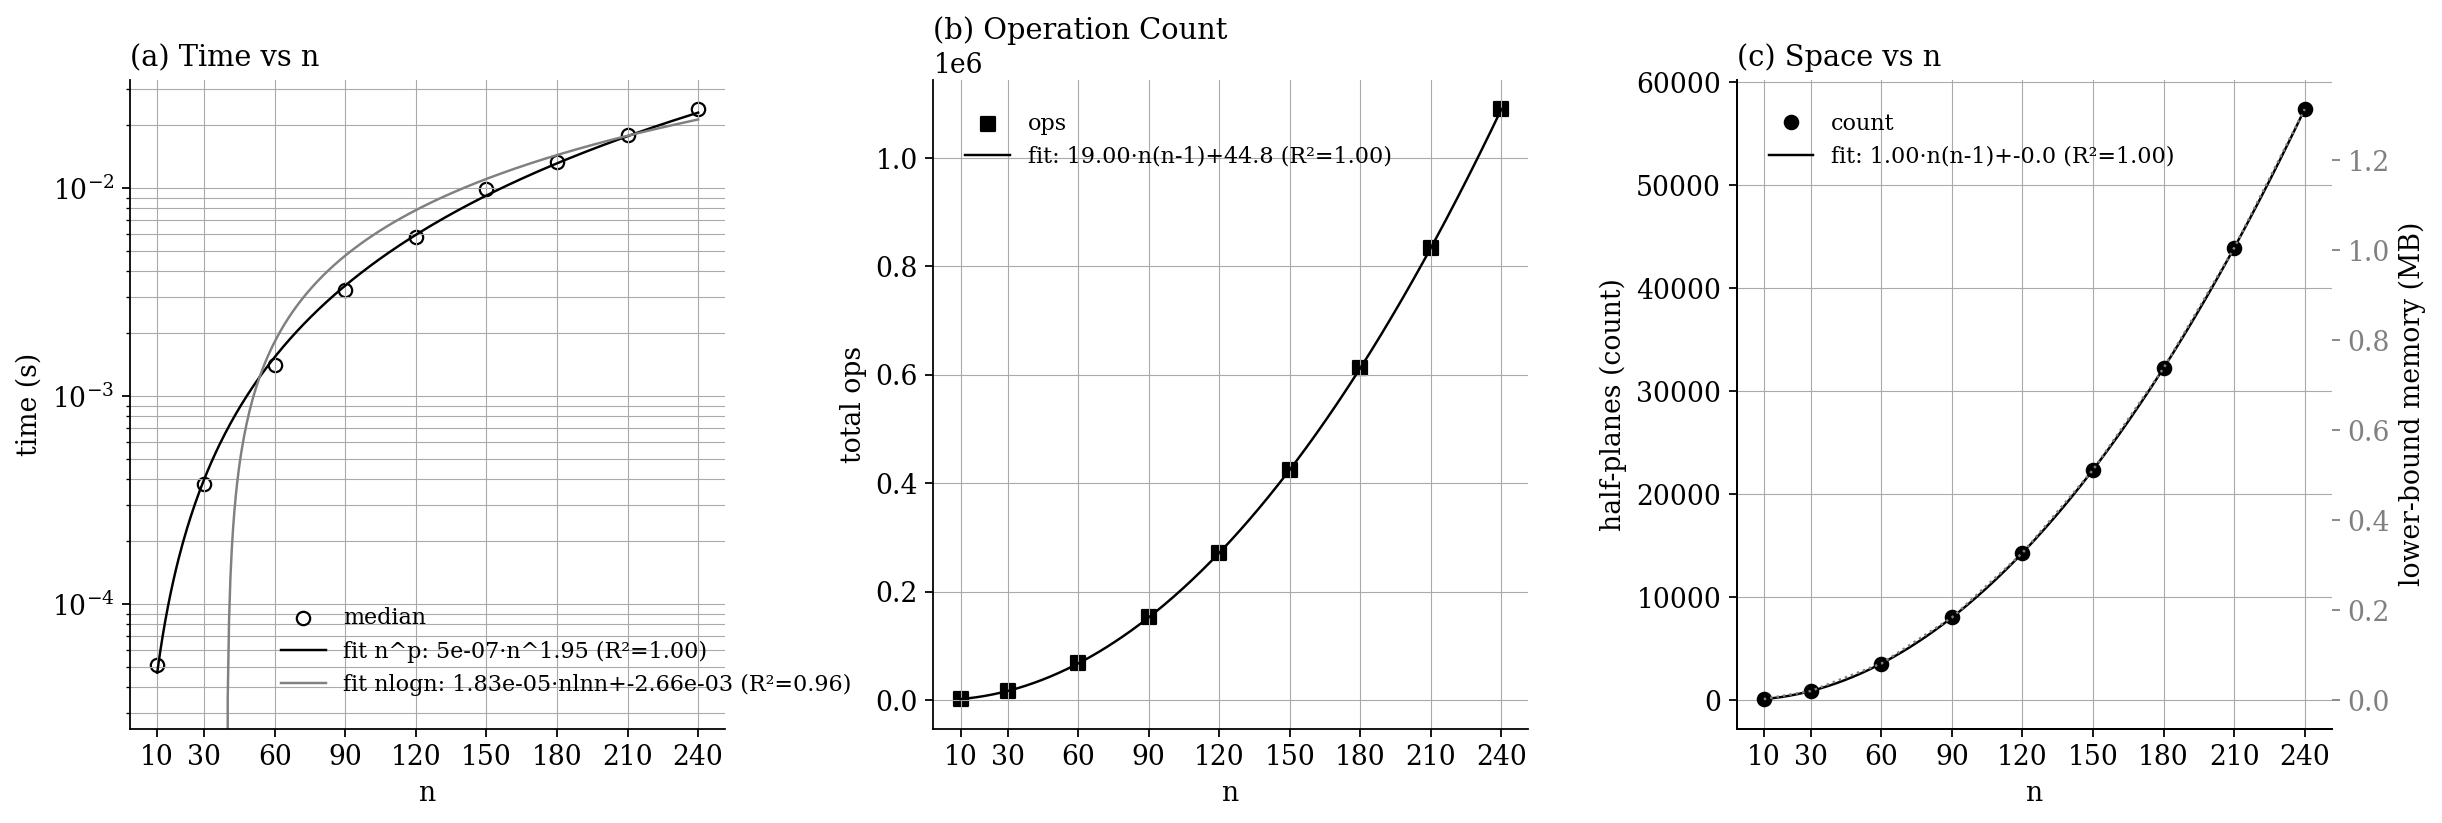
\includegraphics[width=0.95\linewidth]{Pictures/power_complexity2.png}
    \caption{Empirical complexity results for the extended experiment ($n=10$–$240$). 
    (a) Runtime fitted as $T(n)\!\propto\!n^{1.99}$ ($R^2\!=\!1.00$); 
    (b) total operation count $19.0\,n(n-1)+44.8$ ($R^2\!=\!1.00$); 
    (c) half-plane and memory scaling confirming $\Theta(n^2)$ behavior.}
    \label{fig:power_complexity2}
\end{figure}

Overall, the experiments substantiate the theoretical prediction that both computational and storage costs grow quadratically with the number of sites.  
Although small-scale trials were affected by constant-factor noise, extending the input range restored clear $\Theta(n^2)$ scaling in all measures.  
The results confirm that the implemented Power Diagram generator achieves the expected asymptotic behavior, maintaining numerical stability and consistent performance across diverse weighted configurations.

\setcounter{Psec}{0}
\setcounter{Psubsec}{0}
\newpage

\end{document}
